\documentclass[12pt,a4paper]{book}

% --- SOPORTE DE IDIOMA Y MATEMÁTICAS ---
\usepackage[spanish, es-tabla]{babel} % Español y tablas
\usepackage{mathtools}
\usepackage{amsthm}
\usepackage{graphicx}

% Configuramos unicode-math para que no choque con mathtools
\usepackage[
    warnings-off={
        mathtools-colon,    % Silencia el aviso de los dos puntos
        mathtools-overbracket % Silencia el aviso de los brackets
    }
]{unicode-math}

\usepackage{a4wide}

\usepackage[%
  colorlinks=true,
  urlcolor=blue,
  pdfauthor={Jose A. Alonso},%
  pdftitle={Analisis en Lean 4},%
  pdfstartview=FitH,%
  bookmarks=false]{hyperref}

\usepackage{titletoc}

\linespread{1.05}                  % Distancia entre líneas
\raggedbottom                      % No ajusta los espacios verticales.
\setlength{\parskip}{1ex}          % Distancia entre párrfos
\setlength{\parindent}{2em}        % Indentación de comienzo de párrafo
\setcounter{secnumdepth}{3}
\setcounter{tocdepth}{3}

% --- CONFIGURACIÓN DE FUENTES (Crucial para Lean) ---
\usepackage{fontspec}
% Fuente principal para el texto
\setmainfont{Latin Modern Roman}
\setmathfont{Latin Modern Math}
% Fuente para el código Lean (debe soportar Unicode matemático)
\setmonofont{JuliaMono-Regular.ttf}[
    Path = /home/jalonso/.local/share/fonts/juliamono/, % Usa tu ruta absoluta
    Scale = MatchLowercase,
    BoldFont = JuliaMono-Bold.ttf,
    ItalicFont = JuliaMono-RegularItalic.ttf,
    BoldItalicFont = JuliaMono-BoldItalic.ttf
]

% --- CONFIGURACIÓN DE MINTED (Código Lean) ---
\usepackage{minted}
\renewcommand{\MintedPygmentize}{/home/jalonso/.local/bin/pygmentize}
\usemintedstyle{emacs} % Estilo de colores (puedes probar 'friendly' o 'lovelace')
\setminted{
    fontsize=\small,
    breaklines=true,   % Ajustar líneas largas automáticamente
    frame=lines,       % Líneas arriba y abajo del código
    framesep=2mm,
    baselinestretch=1,
    linenos=false      % Cambia a true si quieres números de línea
}

%%%%%%%%%%%%%%%%%%%%%%%%%%%%%%%%%%%%%%%%%%%%%%%%%%%%%%%%%%%%%%%%%%%%%%%%
%% § Cabeceras                                                        %%
%%%%%%%%%%%%%%%%%%%%%%%%%%%%%%%%%%%%%%%%%%%%%%%%%%%%%%%%%%%%%%%%%%%%%%%%

\usepackage{fancyhdr}

\addtolength{\headheight}{\baselineskip}

\pagestyle{fancy}

\cfoot{}

\fancyhead{}
\fancyhead[RE]{\mdseries\sffamily \nouppercase{\leftmark}}
\fancyhead[LO]{\mdseries\sffamily \nouppercase{\rightmark}}
\fancyhead[LE,RO]{\mdseries\sffamily \thepage}

%%%%%%%%%%%%%%%%%%%%%%%%%%%%%%%%%%%%%%%%%%%%%%%%%%%%%%%%%%%%%%%%%%%%%%%%
%% § Definiciones                                                     %%
%%%%%%%%%%%%%%%%%%%%%%%%%%%%%%%%%%%%%%%%%%%%%%%%%%%%%%%%%%%%%%%%%%%%%%%%

\input definiciones

%%%%%%%%%%%%%%%%%%%%%%%%%%%%%%%%%%%%%%%%%%%%%%%%%%%%%%%%%%%%%%%%%%%%%%%%
%% § Título                                                           %%
%%%%%%%%%%%%%%%%%%%%%%%%%%%%%%%%%%%%%%%%%%%%%%%%%%%%%%%%%%%%%%%%%%%%%%%%

\title{{\LARGE Análisis en Lean 4} }
\author{Alex Kontorovich}
\date{Sevilla, \today}

%%%%%%%%%%%%%%%%%%%%%%%%%%%%%%%%%%%%%%%%%%%%%%%%%%%%%%%%%%%%%%%%%%%%%%%%
%% § Documento                                                        %%
%%%%%%%%%%%%%%%%%%%%%%%%%%%%%%%%%%%%%%%%%%%%%%%%%%%%%%%%%%%%%%%%%%%%%%%%

\includeonly{C3-Convergencia_de_sucesiones}

\begin{document}

\maketitle
\newpage

% \noindent
Esta obra está bajo una licencia Reconocimiento--NoComercial--CompartirIgual
2.5 Spain de Creative Commons. 

\vspace*{4ex}

\begin{center}
\fbox{
\begin{minipage}{\textwidth}
\vspace*{1ex}
\noindent                     
{\bf Se permite:}
\begin{itemize}                         
\item copiar, distribuir y comunicar públicamente la obra
\item hacer obras derivadas
\end{itemize}
         
\noindent       
{\bf Bajo las condiciones siguientes:}

\begin{minipage}[t]{20mm}
  \vspace*{0mm}\hspace*{1em}
  
\includegraphics[scale=0.35]{Licencia/deed.png}
\end{minipage}%
\begin{minipage}[t]{14cm}
  \vspace*{0mm}
  {\bf Reconocimiento}. Debe reconocer los créditos de la  obra de la manera
  especificada por el autor.  
\end{minipage}
\\[1ex]

\begin{minipage}[t]{20mm}
  \vspace*{0mm}\hspace*{1em}
  
\includegraphics[scale=0.35]{Licencia/deed-eu.png}
\end{minipage}%
\begin{minipage}[t]{14cm}
  \vspace*{2mm}
  {\bf No comercial}. No puede utilizar esta obra para fines comerciales.
\end{minipage}
\\[1ex]

\begin{minipage}[t]{20mm}
  \vspace*{0mm}\hspace*{1em}
  
\includegraphics[scale=0.35]{Licencia/deed_002.png}
\end{minipage}%
\begin{minipage}[t]{14cm}
  \vspace*{-2mm}
  {\bf Compartir bajo la misma licencia}. Si altera o transforma esta obra, o
  genera una obra derivada, sólo puede distribuir la obra generada bajo una
  licencia idéntica a ésta. 
\end{minipage}

\begin{itemize}    
\item Al reutilizar o distribuir la obra, tiene que dejar bien claro los
  términos de la licencia de esta obra. 
\item Alguna de estas condiciones puede no aplicarse si se obtiene el permiso
 del titular de los derechos de autor.
\end{itemize}
\vspace*{1ex}
\end{minipage}}
\end{center}

\vspace*{4ex}

Esto es un resumen del texto legal (la licencia completa). Para ver una copia
de esta licencia, visite 
\href{http://creativecommons.org/licenses/by-nc-sa/2.5/es/}
     {\url{http://creativecommons.org/licenses/by-nc-sa/2.5/es/}}
o envie una carta a Creative Commons, 559 Nathan Abbott Way, Stanford,
California 94305, USA.

%%% Local Variables: 
%%% mode: latex
%%% TeX-master: t
%%% End: 

% \newpage

\tableofcontents
\clearpage

\chapter{La historia del análisis real}

\section{Preámbulo}

\textbf{SIMPLICIO:} ¿Qué es el ``Análisis real''?

\textbf{SÓCRATES:} Oh, es simplemente Cálculo, pero hecho ``bien''.

\textbf{SIMPLICIO:} ¿Eh? ¿Por qué el Cálculo necesita un nombre nuevo?
¿Qué tiene de malo?

\textbf{SÓCRATES:} Bueno, nada en realidad. Rápido: ¿qué es una
derivada?

\textbf{SIMPLICIO:} ¡Fácil! Si tengo una función $f : \mathbb{R} \to \mathbb{R}$ y es
derivable en $x$, entonces la derivada es:
\[ f'(x) := \lim_{h \to 0} \frac{f(x+h)-f(x)}{h} \]
Esto representa la pendiente ``instantánea'' de la gráfica de la función
$y = f(x)$ en el punto $(x, f(x))$.

\begin{center}
    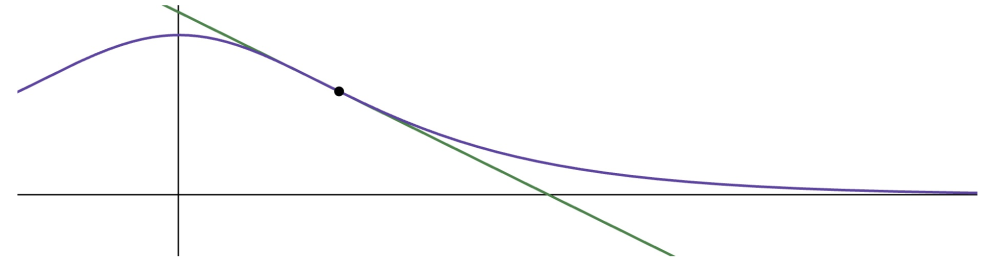
\includegraphics[width=0.5\linewidth]{fig/Derivada.png}
\end{center}

\textbf{SÓCRATES:} ¡Muy bien! Y dime por favor, ¿qué es una integral?

\textbf{SIMPLICIO:} ¡Eso también es fácil! Si quieres integrar nuestra
función $f$ a lo largo de un intervalo, $[a, b]$, por ejemplo, finges
que tienes infinitos rectángulos infinitamente pequeños, calculas sus
áreas como base por altura y los sumas:
\[ \int_{a}^{b} f(x)dx := \lim_{N \to \infty} \sum_{j=1}^{N} \frac{b-a}{N} f\left(a + j\frac{b-a}{N}\right) \]

\begin{center}
    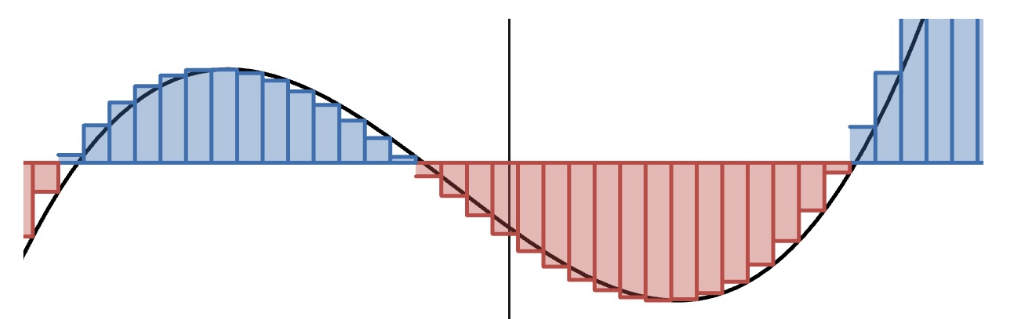
\includegraphics[width=0.5\linewidth]{fig/Integral.png}
\end{center}

\textbf{SÓCRATES:} Estupendo. ¿Y cuáles son los dos Teoremas
Fundamentales del Cálculo?

\textbf{SIMPLICIO:} ¡Estos también son fáciles! El primero dice que si
creas una nueva función integrando $f$ hasta una cantidad variable, $x$,
es decir, defines:
\[ F(x) := \int_{a}^{x} f(t)dt \]
entonces la derivada de la nueva función es simplemente $F'(x) = f(x)$.

\textbf{SÓCRATES:} ¿Y el segundo?

\textbf{SIMPLICIO:} El segundo dice que, a la inversa, si $F$ es una
primitiva de $f$, es decir, $F'(x) = f(x)$, entonces es fácil calcular
el área bajo la curva, porque:
\[ \int_{a}^{b} f(x)dx = F(b) - F(a) \]
¡Así que la derivación y la integración son operaciones inversas!

\textbf{SÓCRATES:} Perfecto. Ahora, aquí está el problema. Has usado
palabras como ``límite'', ``infinitos'', ``infinitamente pequeño'', y
así sucesivamente. ¿Qué significan \textit{realmente}?

\textbf{SIMPLICIO:} Oh, ya sabes, es cuando algo sucede
``eventualmente''. Solo tienes que acostumbrarte a la sensación.

\textbf{SÓCRATES:} Hmm sí, entiendo. Estoy de acuerdo en que esa es una
forma aceptable de pensarlo, al menos por un tiempo, y una que le iba
bien a Newton (que se sentía bastante incómodo con tales palabras) y a
Leibniz (que era más despreocupado en este aspecto), los dos inventores
del cálculo del siglo XVII (si no contamos a personas como los antiguos
griegos Eudoxo y Arquímedes, o al indio Madhava del siglo XIV... pero
esto no es una lección de historia). Leibniz enseñó a los hermanos
Bernoulli (¡los ``primeros estudiantes de bachillerato tecnológico'' del
mundo!), quienes enseñaron, entre otros, al marqués de l'Hôpital y al
gran Leonhard Euler (el primer ``nativo del cálculo''), quien nos enseñó
al resto de nosotros. Todo iba bastante bien... y entonces llegó el
siglo XIX.

\begin{center}
    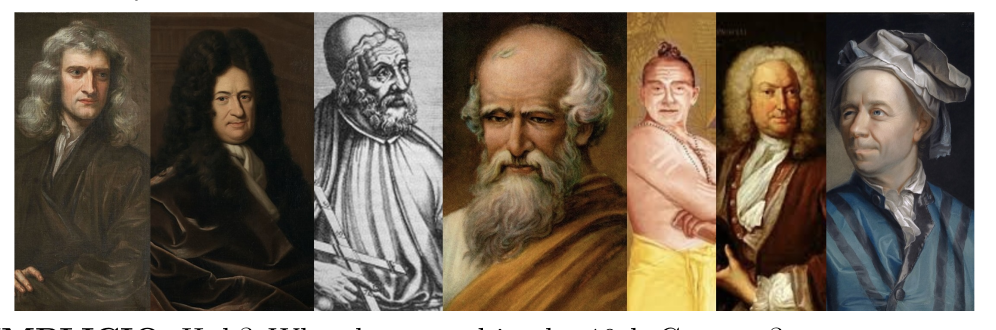
\includegraphics[width=0.5\linewidth]{fig/Matematicos.png}
\end{center}

\textbf{SIMPLICIO:} ¿Eh? ¿Qué pasó en el siglo XIX?

\textbf{SÓCRATES:} Verás, un tipo llamado Augustin-Louis Cauchy apareció
(más o menos en la década de 1810) y empezó a protestar porque no
estábamos haciendo las cosas de forma perfectamente ``rigurosa''. Se
propuso volver a demostrar los teoremas del cálculo usando definiciones
precisas en lugar de explicaciones vagas. Estaba haciendo grandes
progresos, incluyendo la demostración de afirmaciones como: el límite de
funciones continuas es continuo.

\begin{center}
    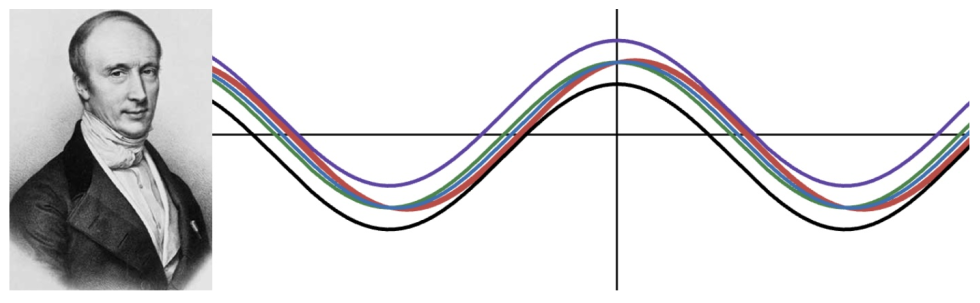
\includegraphics[width=0.5\linewidth]{fig/Cauchy.png}
\end{center}

\textbf{SIMPLICIO:} Claro, eso suena perfectamente razonable. Un límite
es un proceso continuo, así que si se lo aplicas a funciones continuas,
al final deberías obtener algo continuo también. ¿No?

\textbf{SÓCRATES:} Bueno, el problema es que por la misma época, un tipo
llamado Joseph Fourier andaba por ahí afirmando que podía sumar un
montón de senos y cosenos y obtener básicamente cualquier función que
quisiera, ¡incluyendo, por ejemplo, la función discontinua de diente de
sierra!

\textbf{SIMPLICIO:} ¡¿Qué?!

\textbf{SÓCRATES:} Mira tú mismo: aquí tienes una gráfica de
$\sum_{n=1}^{100} \frac{1}{n} \sin(nx)$. A medida que llevas el 100 al
infinito, ¡Fourier afirma que esto se acercará cada vez más a una
función de diente de sierra!

\begin{center}
    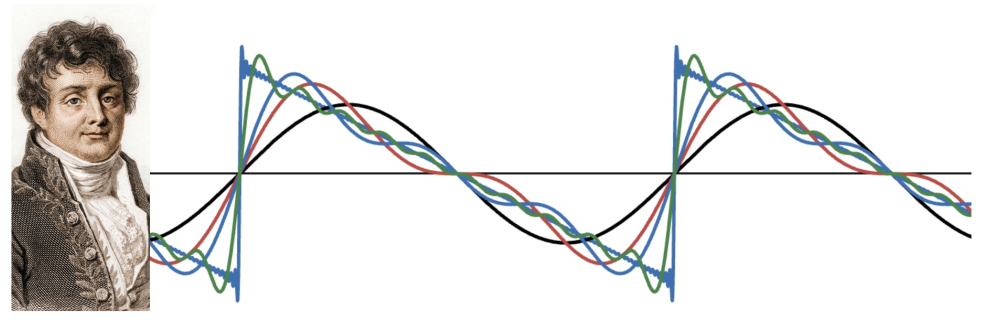
\includegraphics[width=0.5\linewidth]{fig/Fourier.png}
\end{center}

\textbf{SIMPLICIO:} ¡Hala! Espera, se me ocurre un ejemplo aún más
fácil: solo hay que mirar la familia más simple de polinomios, $f_n(x) =
x^n$, en el intervalo unidad $[0, 1]$. Cuando tomas potencias altas de
cualquier punto estrictamente menor que 1, eso tiende a 0 en el límite,
pero las potencias de 1 siempre se mantienen en 1. ¡Así que la función
límite también es discontinua! ¿Qué demonios está pasando aquí?

\begin{center}
    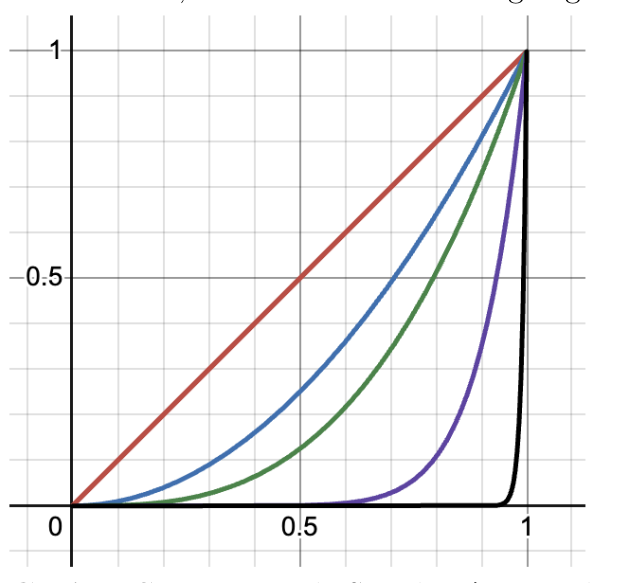
\includegraphics[width=0.5\linewidth]{fig/FamiliaDePolinomios.png}
\end{center}

\textbf{SÓCRATES:} ¡Muy bien, Simplicio! Exactamente, entre Fourier y
Cauchy, ``rompieron las matemáticas''. ¡El que lo rompe, lo paga!

\textbf{SIMPLICIO:} Vale, entonces ¿cuál es la respuesta correcta? ¿Cómo
se hace el cálculo con rigor?

\textbf{SÓCRATES:} ¡No tan rápido! Las cosas se pusieron aún peor, y a
mediados del siglo XIX, ¡la gente se dio cuenta de que ni siquiera
sabíamos qué \textit{son} los números reales!

\textbf{SIMPLICIO:} ¿Qué? ¿Cómo que qué son? Aquí los tienes: está el
cero, y el uno, y el $-2$, y $3/5$, y $\sqrt{2}$, y $e$ y $\pi$. ¿Cuál es
el problema?

\begin{center}
    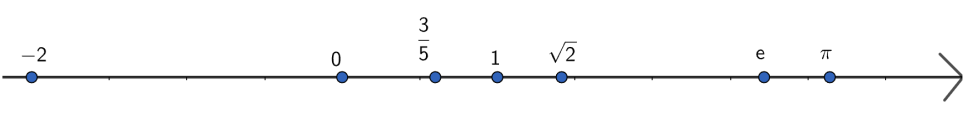
\includegraphics[width=0.5\linewidth]{fig/NumerosReales.png}
\end{center}

\textbf{SÓCRATES:} Bueno, ¿recuerdas que en cálculo necesitas algo
llamado el teorema del valor intermedio?

\textbf{SIMPLICIO:} Claro, si tienes una función continua y pasa de ser
negativa a ser positiva, entonces tiene que cruzar el cero en algún
punto intermedio.

\textbf{SÓCRATES:} Muy bien. Háblame de la función $f : x \mapsto x^2 -
2$. (Decimos: ``$f$ asigna $x$ a $x^2 - 2$''. Observa que escribimos $f
: \mathbb{R} \to \mathbb{R}$ para indicar que $f$ toma números reales y devuelve números
reales, pero sustituimos $\to$ por $\mapsto$ cuando queremos decir qué le ocurre
a una entrada particular $x$ bajo la acción de $f$). En particular, ¿qué
le ocurre a $f$ en los números racionales?

\textbf{SIMPLICIO:} Vale, bueno, si $x$ es un número racional, también
lo es $x^2$, y por tanto también $x^2 - 2$. Así que, en realidad,
podríamos decir que $f : \mathbb{Q} \to \mathbb{Q}$, es decir, $f$ asigna números racionales
a números racionales. Sobre los reales, la gráfica de $y = f(x)$ es una
parábola simple. Pero me habías preguntado por el teorema del valor
intermedio. Hmm. Cuando $x = 0$, sé que $f(0) = 0^2 - 2 = -2$, que es
negativo. Y cuando $x = 2$, $f(2) = 2^2 - 2 = 2$, que es positivo.

\textbf{SÓCRATES:} Continúa...

\textbf{SIMPLICIO:} Así que hay una raíz de $f$ en algún lugar entre 0 y
2. Pero el lugar donde $f$ cruza el eje $x$ es en $x = \sqrt{2} \approx 1.41
\dots$.

\textbf{SÓCRATES:} ¿And what did the Pythagoreans know about this number?

\textbf{SIMPLICIO:} Supuestamente uno de ellos, Hipaso, descubrió que
$\sqrt{2}$ es irracional, lo que arruinó toda su teoría de la geometría
y la forma (originalmente creían que \textit{todos} los números eran
racionales); la leyenda dice que Hipaso fue ahogado en el mar por su
herejía.

\textbf{SÓCRATES:} Entonces...

\textbf{SIMPLICIO:} ¡¿Entonces espera, si nos limitamos a las entradas
racionales, esta parábola es negativa, luego es positiva, y
\textit{nunca} cruza el cero?! Pero hay montones de números racionales
por todas partes. Entonces, ¿qué hace que los números reales sean
diferentes de los números racionales para que el Teorema del Valor
Intermedio sí se cumpla?

\textbf{SÓCRATES:} ¡Ah! Ahora, amigo mío, estamos listos para comenzar.

\section{Introducción a Lean}

\subsection*{Software de demostración de teoremas}

En este curso, utilizaremos un ``asistente de demostración'' llamado
Lean. Se trata de un software que comprueba que nuestras demostraciones
prueban \textit{exactamente} lo que afirmamos que prueban.

\begin{theorem}
Si sabemos que $x = 5$, entonces podemos demostrar que $x = 5$.
\end{theorem}

\begin{minted}{lean}
import Mathlib.Tactic

variable (x : ℝ)

-- 1ª demostración
example
  (h : x = 5)
  : x = 5 :=
by
  exact h

-- 2ª demostración
example
  (h : x = 5)
  : x = 5 :=
by
  apply h

-- 3ª demostración
example
  (h : x = 5)
  : x = 5 :=
by
  assumption
\end{minted}

\textbf{Nota:} Se escribe \texttt{exact h} ya que la hipótesis
\texttt{h} es exactamente lo que queremos demostrar.

\section{La táctica \texttt{rfl}}

\subsection*{Cuando las cosas son idénticas a sí mismas}

A veces, en matemáticas, necesitamos demostrar que algo es igual a sí
mismo. Por ejemplo, demostrar que $x^2 + 2y = x^2 + 2y$. En Lean, usamos
la táctica \texttt{rfl} (abreviatura de \textit{reflexivity}).

\begin{theorem}
Toda expresión matemática es igual a sí misma.
\end{theorem}

\begin{minted}{lean}
import Mathlib.Tactic

variable (x y : ℝ)

-- 1ª demostración
example : x ^ 2 + 2 * y = x ^ 2 + 2 * y :=
by
  rfl

-- 2ª demostración
example : x ^ 2 + 2 * y = x ^ 2 + 2 * y :=
by
  simp
\end{minted}

\section{La táctica \texttt{rw}}

\subsection*{Reescribir con igualdades}

Supongamos que tienes una hipótesis llamada \texttt{Bob : x = 2}, y tu
objetivo es demostrar que $x + y = 2 + y$. Como \texttt{Bob} nos dice
que $x = 2$, podemos sustituir $x$ por 2 usando \texttt{rewrite}.

\begin{theorem}
Si sabemos que $x = 2$, entonces podemos demostrar que $x + y = 2 + y$.
\end{theorem}

\begin{minted}{lean}
-- 1ª demostración
example
  (h : x = 2)
  : x + y = 2 + y :=
by
  rewrite [h]
  -- ⊢ 2 + y = 2 + y
  rfl

-- 2ª demostración
example
  (h : x = 2)
  : x + y = 2 + y :=
by
  subst h
  -- ⊢ 2 + y = 2 + y
  rfl

-- 3ª demostración
example
  (h : x = 2)
  : x + y = 2 + y :=
by
  rw [h]

-- 4ª demostración
example
  (h : x = 2)
  : x + y = 2 + y :=
by
  simp [h]
\end{minted}

\section{La táctica \texttt{ring\_nf}}

\subsection*{Manipulaciones algebraicas}

La táctica \texttt{ring\_nf} (ring normal form) puede realizar
automáticamente expansiones de productos, agrupar términos y aplicar la
propiedad distributiva.

\begin{theorem}
El desarrollo binomial: $(x + y)^3 = x^3 + 3x^2y + 3xy^2 + y^3$.
\end{theorem}

\begin{minted}{lean}
-- 1ª demostración
example : (x + y)^3 = x^3 + 3*x^2*y + 3*x*y^2 + y^3 :=
by
  ring

-- 2ª demostración
example : (x + y)^3 = x^3 + 3*x^2*y + 3*x*y^2 + y^3 :=
by
  ring_nf
\end{minted}

\section{La táctica \texttt{use}}

\subsection*{Demostrar la existencia}

Para demostrar una afirmación existencial ($\exists$), debes proporcionar un
valor específico que funcione usando la táctica \texttt{use}.

\begin{theorem}
  Existe un número real que hace que este desarrollo binomial funcione
  \[ (x + y)^4 = x^4 + 4*x^3*y + c*x^2*y^2 + 4*x*y^3 + y^4 \]
\end{theorem}

\begin{minted}{lean}
example : ∃ c, (x + y)^4 = x^4 + 4*x^3*y + c*x^2*y^2 + 4*x*y^3 + y^4 :=
by
  use 6
  -- ⊢ (x+y)^4 = x^4 + 4*x^3*y + 6*x^2*y^2 + 4*x*y^3 + y^4
  ring
\end{minted}

\section{La táctica \texttt{intro}}

\subsection*{Sentencias universales}

Para demostrar una afirmación ``para todo'' ($\forall$), introducimos un
elemento arbitrario y las hipótesis asociadas usando \texttt{intro}.

\begin{theorem}
Para todos los números reales positivos, se cumple esta identidad
algebraica.
\[(\epsilon + 1)^2 = (\epsilon + 1)^2 \]
\end{theorem}

\begin{minted}{lean}
example : ∀ ε : ℝ, ε > 0 → (ε + 1) ^ 2 = (ε + 1) ^ 2 :=
by
  intro ε h
  -- ε : ℝ
  -- h : ε > 0
  -- ⊢ (ε + 1) ^ 2 = (ε + 1) ^ 2
  rfl
\end{minted}

\section{La táctica \texttt{specialize}}

\subsection*{Uso de sentencias universales}

Si tienes un $\forall$ en una \textbf{hipótesis} y quieres aplicarlo a un
valor específico, usas \texttt{specialize}.

\begin{theorem}
Si una función de $x$ siempre es igual a $x^2$, entonces es igual a $t^2$ cuando se evalúa en $t$.
\end{theorem}

\begin{minted}{lean}
-- 1ª demostración
example
  (t : ℝ)
  (ht : t > 0)
  (f : ℝ → ℝ)
  (hf : ∀ x > 0, f x = x ^ 2)
  : f t = t ^ 2 :=
by
  specialize hf t
  -- hf : t > 0 → f t = t ^ 2
  specialize hf ht
  -- hf : f t = t ^ 2
  exact hf

-- 2ª demostración
example
  (t : ℝ)
  (ht : t > 0)
  (f : ℝ → ℝ)
  (hf : ∀ x > 0, f x = x ^ 2)
  : f t = t ^ 2 :=
by
  apply hf
  -- ⊢ t > 0
  exact ht

-- 3ª demostración
-- ===============

example
  (t : ℝ)
  (ht : t > 0)
  (f : ℝ → ℝ)
  (hf : ∀ x > 0, f x = x ^ 2)
  : f t = t ^ 2 :=
by
  exact hf t ht

-- 4ª demostración
-- ===============

example
  (t : ℝ)
  (ht : t > 0)
  (f : ℝ → ℝ)
  (hf : ∀ x > 0, f x = x ^ 2)
  : f t = t ^ 2 :=
by
  rw [hf]
  -- ⊢ t > 0
  exact ht

-- 5ª demostración
-- ===============

example
  (t : ℝ)
  (ht : t > 0)
  (f : ℝ → ℝ)
  (hf : ∀ x > 0, f x = x ^ 2)
  : f t = t ^ 2 :=
by
  simp_all

-- 6ª demostración
-- ===============

example
  (t : ℝ)
  (ht : t > 0)
  (f : ℝ → ℝ)
  (hf : ∀ x > 0, f x = x ^ 2)
  : f t = t ^ 2 :=
by
  aesop

-- 7ª demostración
-- ===============

example
  (t : ℝ)
  (ht : t > 0)
  (f : ℝ → ℝ)
  (hf : ∀ x > 0, f x = x ^ 2)
  : f t = t ^ 2 :=
by
  solve_by_elim
\end{minted}

\section{El desafío táctico definitivo}

\subsection*{El desafío final}
Aquí tienes la ``Hoja de trucos de los cuantificadores'':

\begin{center}
\begin{tabular}{|l|c|c|}
\hline
Empieza con: & $\forall$ & $\exists$ \\ \hline
\textbf{Objetivo}  & \texttt{intro}      & \texttt{use} \\ \hline
\textbf{Hipótesis} & \texttt{specialize} & \texttt{choose} \\ \hline
\end{tabular}
\end{center}

\begin{theorem}
Dada una función con propiedades específicas, podemos demostrar una
afirmación compleja que implica existencia y universales.
\end{theorem}

\begin{minted}{lean}
-- 1ª demostración
example
  (f : ℝ → ℝ)
  (h1 : ∃ a : ℝ, f a = 3)
  (h2 : ∀ x > 0, f (x + 1) = f x + 9)
  : ∃ b : ℝ, ∀ y > 0, f (y + 1) ^ 2 = (f y + (f b) ^ 2) ^ 2 :=
by
  choose a ha using h1
  -- a : ℝ
  -- ha : f a = 3
  use a
  -- ⊢ ∀ y > 0, f (y + 1) ^ 2 = (f y + f a ^ 2) ^ 2
  intro y hy
  -- y : ℝ
  -- hy : y > 0
  -- ⊢ f (y + 1) ^ 2 = (f y + f a ^ 2) ^ 2
  specialize h2 y hy
  -- h2 : f (y + 1) = f y + 9
  rewrite [h2]
  -- ⊢ (f y + 9) ^ 2 = (f y + f a ^ 2) ^ 2
  rewrite [ha]
  -- ⊢ (f y + 9) ^ 2 = (f y + 3 ^ 2) ^ 2
  ring_nf

-- 2ª demostración
example
  (f : ℝ → ℝ)
  (h1 : ∃ a : ℝ, f a = 3)
  (h2 : ∀ x > 0, f (x + 1) = f x + 9)
  : ∃ b : ℝ, ∀ y > 0, f (y + 1) ^ 2 = (f y + (f b) ^ 2) ^ 2 :=
by
  obtain ⟨a, ha⟩ := h1
  -- a : ℝ
  -- ha : f a = 3
  use a
  -- ⊢ ∀ y > 0, f (y + 1) ^ 2 = (f y + f a ^ 2) ^ 2
  intro y hy
  -- y : ℝ
  -- hy : y > 0
  -- ⊢ f (y + 1) ^ 2 = (f y + f a ^ 2) ^ 2
  rw [h2 y hy]
  -- ⊢ (f y + 9) ^ 2 = (f y + f a ^ 2) ^ 2
  rw [ha]
  -- ⊢ (f y + 9) ^ 2 = (f y + 3 ^ 2) ^ 2
  norm_num

-- 3ª demostración
example
  (f : ℝ → ℝ)
  (h1 : ∃ a : ℝ, f a = 3)
  (h2 : ∀ x > 0, f (x + 1) = f x + 9)
  : ∃ b : ℝ, ∀ y > 0, f (y + 1) ^ 2 = (f y + (f b) ^ 2) ^ 2 :=
by
  obtain ⟨a, ha⟩ := h1
  -- a : ℝ
  -- ha : f a = 3
  use a
  -- ⊢ ∀ y > 0, f (y + 1) ^ 2 = (f y + f a ^ 2) ^ 2
  grind

-- 4ª demostración
example
  (f : ℝ → ℝ)
  (h1 : ∃ a : ℝ, f a = 3)
  (h2 : ∀ x > 0, f (x + 1) = f x + 9)
  : ∃ b : ℝ, ∀ y > 0, f (y + 1) ^ 2 = (f y + (f b) ^ 2) ^ 2 :=
by
  rcases h1 with ⟨a, ha⟩
  -- a : ℝ
  -- ha : f a = 3
  use a
  -- ⊢ ∀ y > 0, f (y + 1) ^ 2 = (f y + f a ^ 2) ^ 2
  grind
\end{minted}

\section*{Epílogo}

¡Victoria! Has completado un argumento matemático genuinamente
sofisticado. Usar un demostrador de teoremas es como aprender ajedrez:
es mucho más fácil ver el tablero que leer solo la notación. Esta
retroalimentación inmediata construye la intuición necesaria para el
cálculo riguroso.

%%% Local Variables:
%%% mode: latex
%%% TeX-master: "Analisis_en_Lean"
%%% End:

\chapter{El cálculo de $\pi$ de Newton}

\section{La revolución matemática de 1666}

\noindent \textbf{SIMPLICIO:} He oído que Newton tenía una forma muy
ingeniosa de calcular $\pi$. ¿Podría hablarme de ello?

\noindent \textbf{SÓCRATES:} Por supuesto. Todo empieza alrededor de
1665-1666, cuando Newton estaba a punto de cumplir 23 años. ¿Recuerdas
algo significativo sobre ese año?

\noindent \textbf{SIMPLICIO:} ¿No es ese el \textit{``annus mirabilis''}
de Newton, su año de los milagros? Si mal no recuerdo, se vio obligado a
abandonar Cambridge debido a un brote de la Gran Peste, y realizó sus
descubrimientos más trascendentales (cálculo, óptica, gravitación, etc.)
mientras guardaba cuarentena en aislamiento en su casa familiar de
Woolsthorpe.

\noindent \textbf{SÓCRATES:} Exactamente. Y una de las primeras cosas
que descubrió en ese año fue una nueva versión del teorema del
binomio. Dime, por favor, ¿qué se puede decir sobre $(1 + x)^n$?

\noindent \textbf{SIMPLICIO:} Claro, si desarrollas $(1 + x)^n$, obtienes:
\[ \binom{n}{0} + \binom{n}{1}x + \binom{n}{2}x^2 + \dots + \binom{n}{n}x^n \]
\noindent Aquí $\binom{n}{k}$ es el ``coeficiente binomial'', el número
de formas de elegir $k$ objetos de un conjunto de $n$. Explícitamente,
$\binom{n}{k} = \frac{n!}{k!(n-k)!}$. Estos son simplemente los números
del triángulo de Pascal, y puedes leer fácilmente la fila $n$-ésima.

\begin{center}
    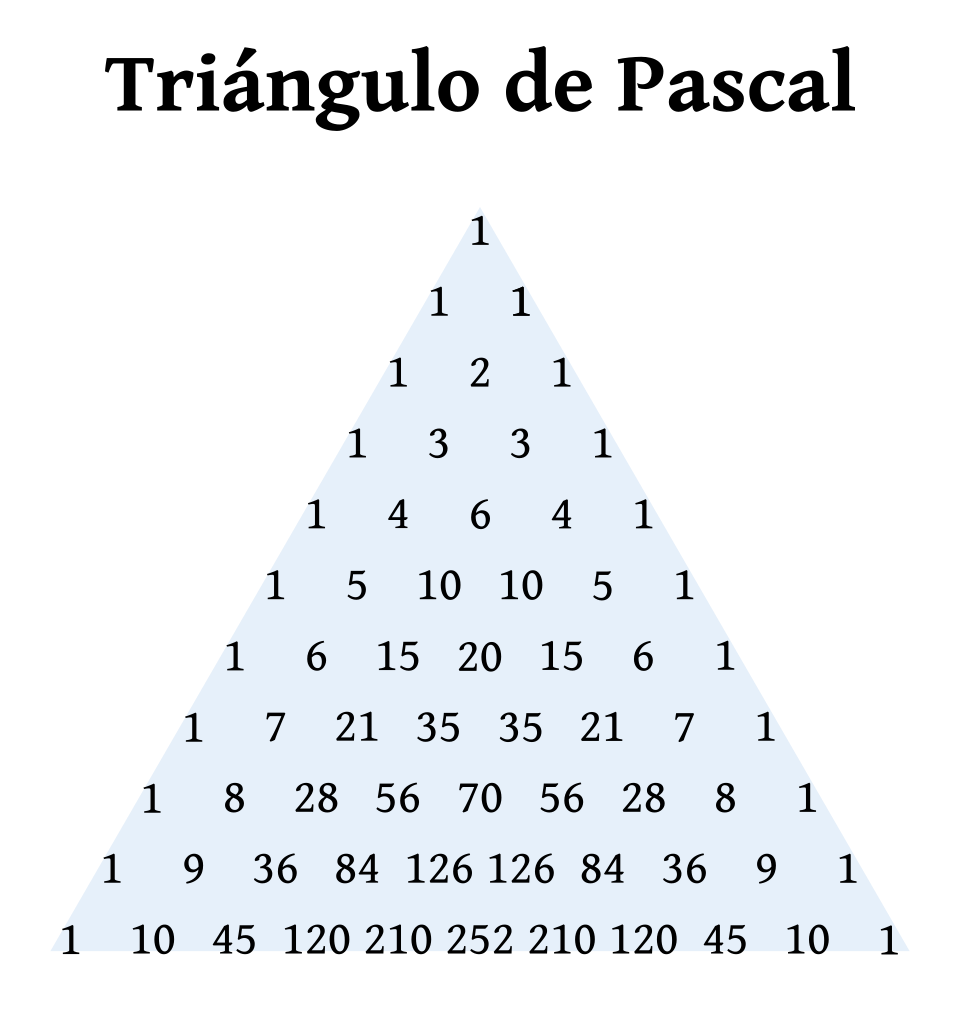
\includegraphics[width=0.5\linewidth]{fig/Triangulo_de_Pascal.png}
\end{center}

\noindent \textbf{SÓCRATES:} ¡Excelente! ¿Y conoces la notación sigma?

\noindent \textbf{SIMPLICIO:} Creo que sí. Podría haber escrito lo mismo
como $\sum_{k=0}^{n} \binom{n}{k} x^k$. En general, si tienes una función
$f : \mathbb{N} \to \mathbb{R}$ y quieres expresar
$f(a) + f(a + 1) + \dots + f(b)$, es decir, la suma de $f(k)$ mientras
$k$ varía desde un entero $a$ hasta otro entero $b$, puedes escribirlo
como $\sum_{k=a}^{b} f(k)$.

\noindent \textbf{SÓCRATES:} Muy bien. Así que tenemos
$(1 + x)^n = \sum_{k=0}^{n} \binom{n}{k} x^k$. Ahora, ¿me permitirías
escribir esto como una suma que llegue hasta el infinito?
\[ (1 + x)^n = \sum_{k=0}^{\infty} \binom{n}{k} x^k \]

\noindent \textbf{SIMPLICIO:} Hmm. Vale, creo que entiendo a qué te
refieres: el triángulo de Pascal tiene ceros implícitos en todas partes
por fuera, así que $\binom{n}{k}$ es simplemente cero en cuanto $k >
n$. Así que lo has escrito como una suma infinita, aunque secretamente
termina tras un número finito de términos. Pero, ¿para qué sirve
extenderla así?

\noindent \textbf{SÓCRATES:} Bueno, déjame preguntarte esto: ¿se te
ocurre alguna forma de dar sentido a esta fórmula cuando $n = -1$?

\noindent \textbf{SIMPLICIO:} ¡¿Cómo?! No puedes usar coeficientes
binomiales. ¡¿Cómo vas a elegir 3 cosas de un conjunto de $-1$?! ¡Eso no
tiene sentido!

\noindent \textbf{SÓCRATES:} Tienes razón, pero muchos de los grandes
descubrimientos en matemáticas ocurren cuando te das cuenta de que
puedes ``romper las reglas'' y seguir un patrón más allá de su límite
previsto. Ponte en el lugar de Newton; ¿qué se le ocurriría a un genio
como él?

\noindent \textbf{SIMPLICIO:} Bueno, tenemos esta otra fórmula para los
coeficientes binomiales, no en términos combinatorios, sino con
factoriales: $\binom{n}{k} = \frac{n!}{k!(n-k)!}$. Eso sigue sin ayudar
porque, ¡¿qué demonios se supone que es $(-1)!$?! ¡Ah, espera! También
podemos escribirlo así:
\[ \binom{n}{k} = \frac{n(n - 1)(n - 2) \dots (n - k + 1)}{k!} \] Y de
esta manera, ``esquivamos'' el problema de lidiar con $(-1)!$ y pasamos
directamente a números ``normales''.

\noindent \textbf{SÓCRATES:} ¿Podrías escribir esto usando la notación
de productorio?

\noindent \textbf{SIMPLICIO:} Claro, es como la notación de sumatorio
pero con una $\Pi$:
\[ \binom{n}{k} = \frac{1}{k!} \prod_{\ell=1}^{k} (n - \ell) \]

\noindent \textbf{SÓCRATES:} ¡Vaya! ¿Estás seguro de los límites de ese
producto?

\noindent \textbf{SIMPLICIO:} ¡Argh! Es tan fácil cometer un error
tonto. Después de escribir la fórmula, debería haber comprobado que los
valores de inicio y fin fueran correctos; el contador $\ell$ debería ir de
$0$ a $k - 1$, no de $1$ a $k$. ¿Así mejor?
\[ \binom{n}{k} = \frac{1}{k!} \prod_{\ell=0}^{k-1} (n - \ell) \]

\noindent \textbf{SÓCRATES:} Perfecto. Continúa.

\noindent \textbf{SIMPLICIO:} Vale, si aceptamos seguir este patrón,
obtenemos:
\begin{itemize}
\item $\binom{-1}{0} = 1$, lo cual tiene sentido porque cualquier fila
  del triángulo de Pascal empieza por $1 = \binom{c}{0}$.
\item $\binom{-1}{1} = (-1)/1! = -1$, que también tiene sentido porque
  el siguiente término en la ``fila $c$'' es siempre $\binom{c}{1} = c$.
\item $\binom{-1}{2} = (-1)(-2)/2! = +1$.
\item $\binom{-1}{3} = (-1)(-2)(-3)/3! = -1$.
\end{itemize}
Ya veo el patrón: simplemente alterna entre $+1$ y $-1$, así que la
serie queda:
\[ (1 + x)^{-1} = 1 - x + x^2 - x^3 + x^4 - x^5 + \dots \]

\noindent \textbf{SÓCRATES:} ¡Muy bien! Pero, ¿tiene esta fórmula algún
sentido real? ¿Cómo podrías ponerla a prueba?

\noindent \textbf{SIMPLICIO:} Vale, si se supone que esa serie
``representa'' a $1/(1 + x)$, entonces si multiplico todo por $(1 + x)$,
debería obtener simplemente $1$. Vamos a probar:
\[ (1 + x)(1 - x + x^2 - x^3 + x^4 - x^5 + \dots) = ? \]
Primero multiplicaré todo por $1$, luego por $x$, y los sumaré.
\[ (1 - x + x^2 - x^3 + x^4 - x^5 + \dots) + (x - x^2 + x^3 - x^4 + x^5 \dots) \]
Si reordeno los términos, todo se cancela y solo queda el $1$
inicial. ¡Genial!

\noindent \textbf{SÓCRATES:} Interesante. ¿Y se te ``permite'' reordenar
los términos así?

\noindent \textbf{SIMPLICIO:} Bueno... ¿por qué no?

\noindent \textbf{SÓCRATES:} Olvídalo por ahora; pareces satisfecho con
que tenga sentido decir que la serie
$1 - x + x^2 - x^3 + x^4 - x^5 + \dots$ ``converge'' (sea lo que sea que
eso signifique) a $(1 + x)^{-1}$.

\noindent \textbf{SIMPLICIO:} Pensándolo bien, ya sabía esto; ¡es solo
la serie geométrica! Sé que
$1 + \lambda + \lambda^2 + \lambda^3 + \dots$ suma $1/(1 - \lambda)$, y nuestra serie
simplemente reemplaza $\lambda$ por $-x$.

\noindent \textbf{SÓCRATES:} Sí, muy bien. ¿Y dónde podría ``encajar''
esto en el triángulo de Pascal?

\noindent \textbf{SIMPLICIO:} ¡Cielos! ¿Acabamos de descubrir una
extensión del triángulo que va hacia ``arriba''?

\begin{center}
    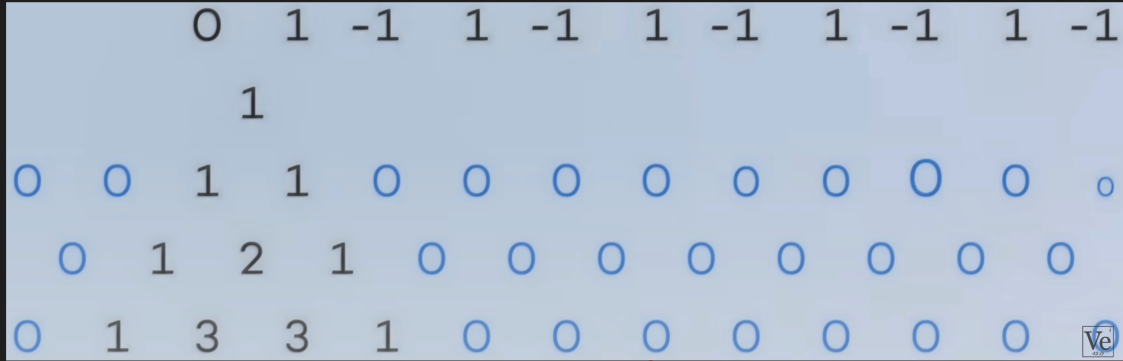
\includegraphics[width=0.5\linewidth]{fig/Triangulo_de_Pascal_arriba.png}
\end{center}

\noindent \textbf{SÓCRATES:} En efecto, y de hecho podemos continuar
este patrón para $n = -2, -3, -4$, y así sucesivamente. Te dejaré que lo
deduzcas tú mismo, ¡pero en realidad obtenemos todo otro Triángulo de
Pascal (con algunos signos negativos) por encima del estándar!

\begin{center}
    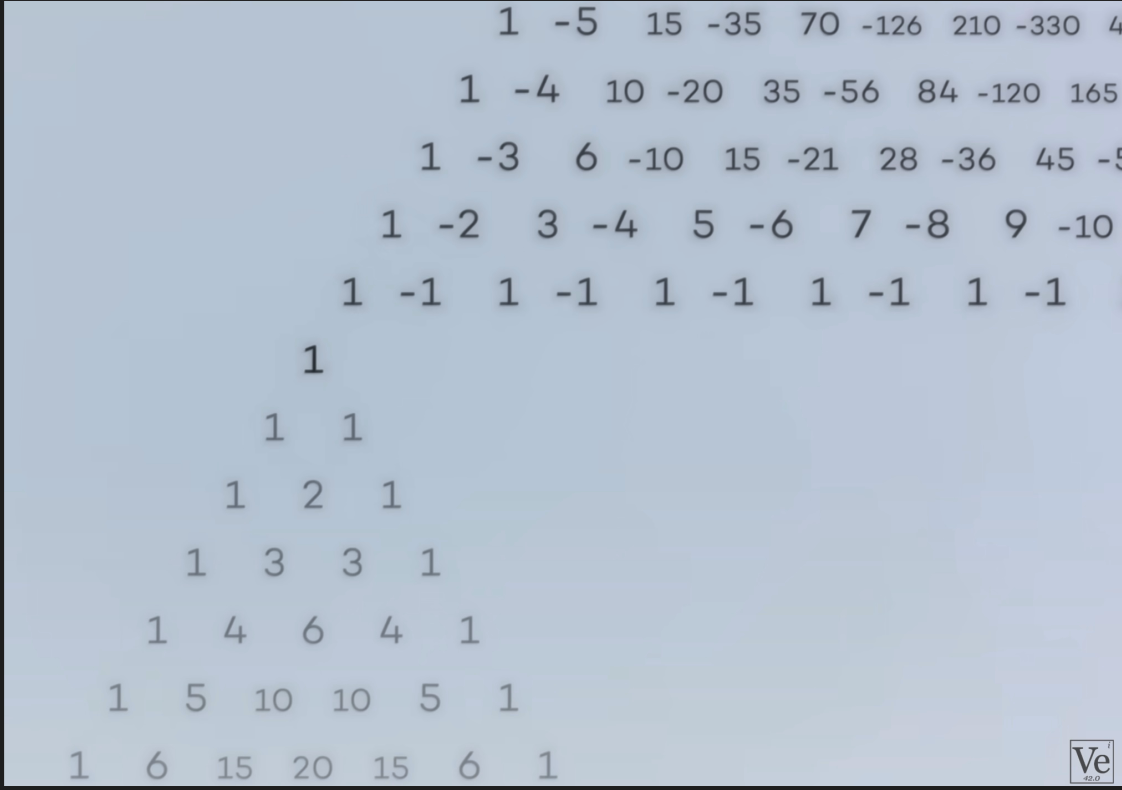
\includegraphics[width=0.5\linewidth]{fig/Triangulo_de_Pascal_extendido.png}
\end{center}

\noindent ¿Ves cómo sigue cumpliendo la regla habitual de que los dos
números de arriba sumen el valor que tienen justo debajo? Pero probemos
algo aún más exótico. ¿Puedes hacer que el Teorema del Binomio funcione
para $n = 1/2$?

\noindent \textbf{SIMPLICIO:} ¡Hala! ¿$n = 1/2$? Eso es... ¡forzar mucho
las cosas! Pero déjame intentar usar la misma fórmula. Así que
$\binom{1/2}{k} = \frac{1}{k!} \prod_{\ell=0}^{k-1} (1/2 - \ell)$. Voy a calcular
los primeros términos:
\begin{itemize}
\item $\binom{1/2}{0} = 1$ (como siempre).
\item $\binom{1/2}{1} = (1/2)/1! = 1/2$ (de nuevo, coincide con el
  patrón que ya conocíamos).
\item $\binom{1/2}{2} = (1/2)(-1/2)/2! = -1/8$.
\item $\binom{1/2}{3} = (1/2)(-1/2)(-3/2)/3! = 1/16$.
\item $\binom{1/2}{4} = \frac{(1/2)(-1/2)(-3/2)(-5/2)}{4!} = -5/128$.
\end{itemize}
Así que $(1 + x)^{1/2} = 1 + \frac{1}{2}x - \frac{1}{8}x^2 + \frac{1}{16}x^3 - \frac{5}{128}x^4 + \dots$\\
Pero espera... ¡¿se supone que esto es $\sqrt{1 + x}$?!

\noindent \textbf{SÓCRATES:} De nuevo, entra en la mente de Newton:
¿cómo podría él justificar si esta fórmula tiene algún sentido?

\noindent \textbf{SIMPLICIO:} ¡Ah, ya veo! Si elevamos la fórmula al
cuadrado y lo multiplicamos todo, supongo que deberíamos obtener
$1 + x$; eso justificaría llamar a la serie $\sqrt{1 + x}$.

\noindent \textbf{SÓCRATES:} ¡Adelante!

\noindent \textbf{SIMPLICIO:} Vale, quiero calcular:
\[ \left( 1 + \frac{1}{2}x - \frac{1}{8}x^2 + \frac{1}{16}x^3 - \frac{5}{128}x^4 + \dots \right)^2 \]
Eso significa elevar cada término al cuadrado, y también añadir el doble
de cada producto de pares distintos de términos.

\noindent \textbf{SÓCRATES:} Correcto. ¿Se te ocurre una buena forma de
llevar la cuenta de todo?

\noindent \textbf{SIMPLICIO:} ¡Oh, ya sé! Vamos a agrupar las cosas por
la potencia de $x$ involucrada. La primera es fácil: $x^0 = 1$, que solo
se obtiene elevando al cuadrado el primer término. Así que ese
coeficiente es $1$.
\\
Para el coeficiente de $x^1$, no puedo elevar al cuadrado nada que
contenga $x$, así que solo puedo multiplicar el término en $x$ por el
término constante y, por supuesto, duplicarlo. Eso es simplemente
$2 \times 1 \times \frac{1}{2}x = x$. Así que el coeficiente de $x$ es $1$.
\\
Para $x^2$, obtengo dos contribuciones: de constante por cuadrático,
$2 \times 1 \times (-\frac{1}{8}x^2) = -\frac{1}{4}x^2$, y también del cuadrado
del término lineal: $(\frac{1}{2}x)^2 = \frac{1}{4}x^2$. Así que el
coeficiente total es $-\frac{1}{4} + \frac{1}{4} = 0$.
\\
Probemos unos pocos más. Para obtener $x^3$, necesito:
\begin{itemize}
    \item $2 \times 1 \times \frac{1}{16}x^3 = \frac{1}{8}x^3$ (constante por el término $x^3$)
    \item $2 \times \frac{1}{2}x \times (-\frac{1}{8}x^2) = -\frac{1}{8}x^3$ (el término $x$ por el término $x^2$)
\end{itemize}
Así que el coeficiente total de $x^3$ es $\frac{1}{8} - \frac{1}{8} = 0$.
\\
¡Esto es increíble! Parece que todos los términos de orden superior se
cancelan perfectamente. Apuesto a que eso seguirá pasando y el cuadrado
resultará ser exactamente $1 + x$; ¡la fórmula realmente funciona!
\\
Pero espera, ¡¿ahora tenemos otra fila entera en el triángulo de Pascal,
entre las filas 0 y 1?!

\begin{center}
    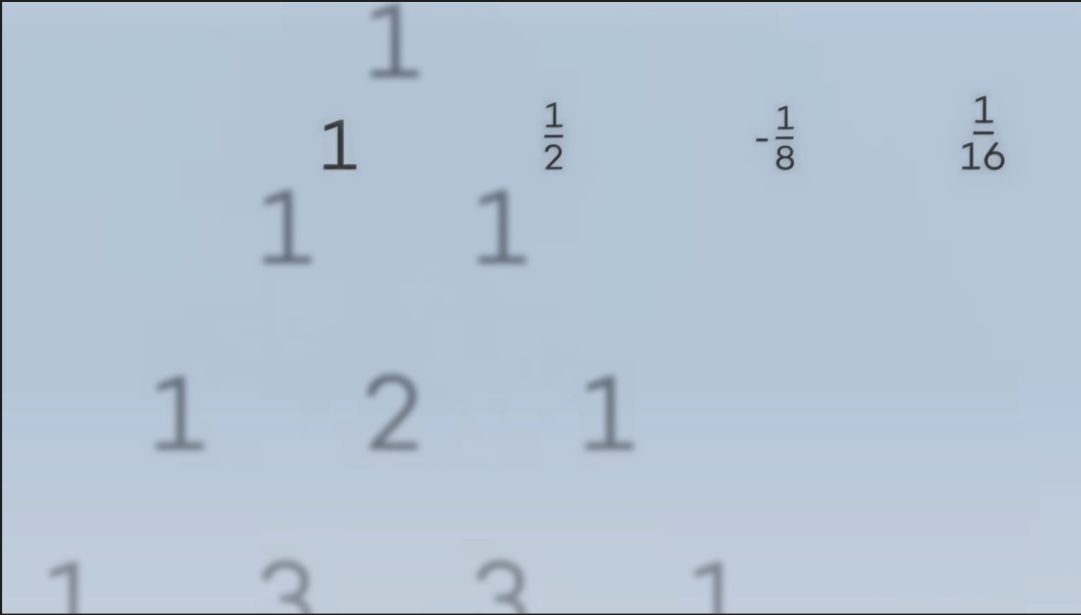
\includegraphics[width=0.5\linewidth]{fig/Triangulo_de_Pascal_racional.png}
\end{center}

\noindent \textbf{SÓCRATES:} Hermoso, ¿verdad?

\noindent \textbf{SIMPLICIO:} Espera, esto es mucho más sencillo de lo
que parece. ¿No es esto simplemente lo mismo que el desarrollo de Taylor
alrededor de $x = 0$ de la función $f(x) = \sqrt{1 + x}$? Ya sé cómo
hacer eso por mis clases de Cálculo.

\noindent \textbf{SÓCRATES:} Sí, muy bien; pero Brook Taylor (el de las
series de Taylor) no demostró su teorema general hasta 1715, unas
décadas después del cálculo de $\pi$ de Newton.

\noindent \textbf{SÓCRATES:} Ahora, supón que quisieras calcular algo
como $\sqrt{3}$. ¿Se te ocurre alguna forma de hacerlo usando esta
fórmula?

\noindent \textbf{SIMPLICIO:} Hmm, la función es $\sqrt{1 + x}$, así que
supongo que quiero poner $x = 2$. Entonces obtengo:
\[ \sqrt{1 + 2} = 1 + \frac{1}{2}(2) - \frac{1}{8}(2)^2 + \frac{1}{16}(2)^3 - \frac{5}{128}(2)^4 + \dots \]
Sumar estos cinco términos da $11/8 = 1,375$, que no está muy cerca de
$\sqrt{3} \approx 1,73$. Además, los términos individuales no son tan
pequeños; por ejemplo, el último es $\frac{5}{128}(2)^4 = 5/8 = 0,625$.

\noindent \textbf{SÓCRATES:} Bueno, claro, si eliges una $x$ grande,
como $x > 1$, entonces las potencias de $x$ son cada vez más grandes (¡y
exponencialmente!). ¿Se te ocurre alguna otra cosa que pudieras hacer?

\noindent \textbf{SIMPLICIO:} ¡Ah, ya veo! Sé que $3$ está cerca de $4$,
que es un cuadrado perfecto. ¿Y si escribimos:
\[ \sqrt{3} = \sqrt{4 - 1} = \sqrt{4(1 - 1/4)} = 2\sqrt{1 - 1/4} \]
Así que ahora, si aplico nuestra fórmula con $x = -1/4$ (¡que es menor
que uno!), supongo que obtendré:
\[ \sqrt{3} \approx 2 \left( 1 + \frac{1}{2}(-1/4) - \frac{1}{8}(-1/4)^2 + \frac{1}{16}(-1/4)^3 - \frac{5}{128}(-1/4)^4 + \dots \right) \]
Tomando solo estos cinco términos, la fracción de la derecha sale
$28379/16384 \approx 1,73212$, que es impresionantemente cercana a $\sqrt{3} \approx
1,7320508$. ¡Hemos obtenido 3 decimales de precisión, nada mal!

\noindent \textbf{SÓCRATES:} ¡Genial! Ahora ves el poder del Teorema del
Binomio de Newton. Vale, volvamos entonces a tu pregunta original sobre
la estimación de $\pi$ de Newton.

\noindent \textbf{SIMPLICIO:} Hmmm, $\pi$ es la relación entre la
circunferencia y el diámetro de un círculo. Pero, ¿de dónde voy a sacar
una longitud?

\noindent \textbf{SÓCRATES:} ¡Ah! Pero, ¿qué aprendimos de Arquímedes?

\noindent \textbf{SIMPLICIO:} ¡Oh! Que $\pi$ también es un \textit{área},
no solo una longitud. Es el área de un círculo unidad $\pi r^2$ donde
$r = 1$.

\noindent \textbf{SÓCRATES:} Precioso. ¿Y podrías encontrar el área de
un círculo escondida en alguna parte?

\noindent \textbf{SIMPLICIO:} ¡Creo que lo veo! Gracias a Descartes y a
las coordenadas ``cartesianas'', podemos expresar el círculo como la
gráfica de $x^2 + y^2 = 1$, o para convertirlo en una función,
$y = \sqrt{1 - x^2}$. Así que solo tenemos que reemplazar $x$ en nuestra
serie por $-x^2$.
\[ \sqrt{1 - x^2} = 1 + \frac{1}{2}(-x^2) - \frac{1}{8}(-x^2)^2 + \frac{1}{16}(-x^2)^3 - \frac{5}{128}(-x^2)^4 + \dots \]
\[ = 1 - \frac{x^2}{2} - \frac{x^4}{8} - \frac{x^6}{16} - \frac{5x^8}{128} - \dots \]
Y el área bajo la curva $y = \sqrt{1 - x^2}$ desde $x = 0$ hasta $x = 1$
es un cuarto de círculo.

\begin{center}
    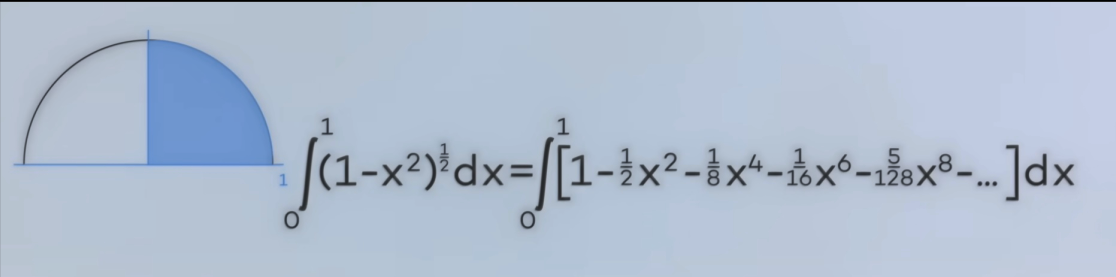
\includegraphics[width=0.5\linewidth]{fig/Area_del_circulo.png}
\end{center}

\noindent \textbf{SÓCRATES:} ¡Por suerte, Newton acababa de inventar el
cálculo! Entonces, ¿de qué otra forma podría calcular el área bajo esta
curva?

\noindent \textbf{SIMPLICIO:} ¡Con una integral! Así que:
\[ \frac{\pi}{4} = \int_{0}^{1} \sqrt{1 - x^2} \, dx = \int_{0}^{1} \left( 1 - \frac{x^2}{2} - \frac{x^4}{8} - \frac{x^6}{16} - \frac{5x^8}{128} - \dots \right) dx \]
Simplemente integraré término a término...

\noindent \textbf{SÓCRATES:} ¡Epa, espera un momento! ¿Por qué se te
permite...? Sabes qué, da igual, lo siento. Adelante.

\noindent \textbf{SIMPLICIO:} Qué raro eres. En fin. Integrando término
a término obtengo:
\[ \frac{\pi}{4} = \left[ x - \frac{x^3}{6} - \frac{x^5}{40} - \frac{x^7}{112} - \frac{5x^9}{1152} - \dots \right]_{0}^{1} \]
\[ = 1 - \frac{1}{6} - \frac{1}{40} - \frac{1}{112} - \frac{5}{1152} - \dots \]
¡Vaya! ¡Así que Newton obtuvo una serie infinita para $\pi$! Si evalúo solo estos cinco términos y multiplico por 4, obtengo la fracción $32057/10080 \approx 3,180$. ¡No está mal!

\noindent \textbf{SÓCRATES:} No está mal, en efecto. Sabes, Simplicio,
muchos artículos de matemáticas tienen prácticamente cero ideas nuevas;
simplemente hacen algo que nadie se molestó en hacer antes en un
contexto ligeramente distinto. Un artículo de matemáticas realmente
bueno puede tener una o dos ideas genuinamente nuevas. ¡Newton ya va por
la idea nueva número cinco, y aún no ha terminado!

\noindent \textbf{SIMPLICIO:} Vale, ¿y cuál es la idea nueva número
seis?

\noindent \textbf{SÓCRATES:} Bueno, ¿recuerdas que integraste hasta
$x = 1$? En tu serie,
\[ \frac{\pi}{4} = \left[ x - \frac{x^3}{6} - \frac{x^5}{40} - \frac{x^7}{112} - \frac{5x^9}{1152} - \dots \right]_{0}^{1} \]
tienes todas estas potencias altas de $x$, pero se están
``desperdiciando'' porque estás poniendo $x = 1$. ¿Y si en su lugar solo
integraras hasta, por ejemplo, $x = 1/2$?

\noindent \textbf{SIMPLICIO:} ¡Ah, qué guay! Entonces la serie
convergerá mucho más rápido. Pero espera, eso cambia la geometría. En
lugar de un cuarto de círculo, ahora tenemos... un sector de 30 grados,
que tiene un área de $\pi/12$, más un triángulo 30-60-90 (¡ah, por eso
sugeriste $x = 1/2$!) con área
$\frac{1}{2} \times \frac{1}{2} \times \frac{\sqrt{3}}{2}$.

\begin{center}
    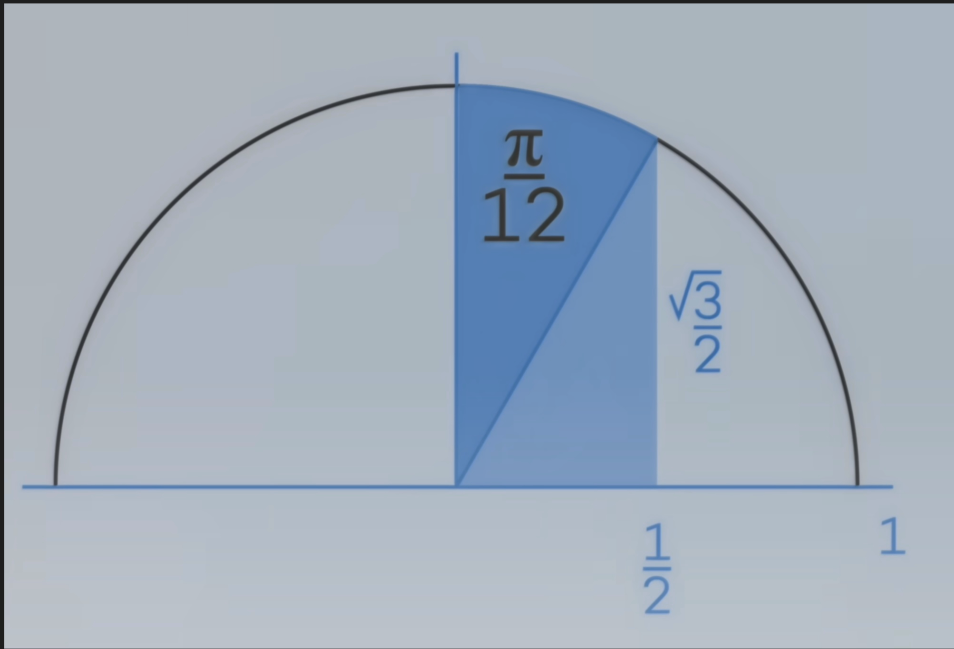
\includegraphics[width=0.5\linewidth]{fig/Circulo_sector_y_triangulo.png}
\end{center}

\noindent ¡Menos mal que ya sabemos cómo estimar $\sqrt{3}$ rápidamente
con gran precisión! (Esa es la contrapartida: podríamos elegir una $x$
aún más pequeña para una convergencia más rápida, pero entonces
tendríamos que lidiar con evaluaciones geométricas cada vez más
complicadas; así que $x = 1/2$ es el ``punto ideal''). Así que ahora:
\[ \frac{\pi}{12} + \frac{\sqrt{3}}{8} = \left[ x - \frac{x^3}{6} - \frac{x^5}{40} - \frac{x^7}{112} - \frac{5x^9}{1152} - \dots \right]_{0}^{1/2} \]
\[ = \frac{1}{2} - \frac{1}{6} \left(\frac{1}{2}\right)^3 - \frac{1}{40} \left(\frac{1}{2}\right)^5 - \frac{1}{112} \left(\frac{1}{2}\right)^7 - \frac{5}{1152} \left(\frac{1}{2}\right)^9 - \dots \]
Evaluando de nuevo solo estos cinco términos obtenemos la fracción
$9874097/20643840$. Y ahora, aislando $\pi$ obtenemos la estimación:
\[ \pi \approx 12 \times \left( 9874097/20643840 - \frac{\sqrt{3}}{8} \right) \approx 3,14161, \]
que solo difiere en dos partes por cada 100.000 de la estimación real $\pi
\approx 3,14159$. ¡Y todo eso con solo cinco términos, increíble!

\noindent \textbf{SÓCRATES:} Sí, Newton fue realmente
impresionante. Aquí tienes un buen vídeo de YouTube de Veritasium que
analiza toda esta saga: \url{https://youtu.be/gMlf1ELvRzc}

\noindent De hecho, una serie para $\pi$ similar a esta fue descubierta
dos siglos antes por el matemático indio Madhava de Sangamagrama. Y
harían falta dos siglos más hasta que los matemáticos descubrieran cómo
justificar rigurosamente el trabajo de Newton. Para hacerlo, tuvieron
que averiguar:
\begin{itemize}
\item ¿Qué significa que una sucesión de números reales
  $a_0, a_1, a_2, \dots$ converja?
\item ¿Qué significa que una serie (es decir, una sucesión de sumas
  parciales) $a_0 + a_1 + a_2 + \dots$ converja, y podríamos sumar estos
  números en cualquier orden que quisiéramos?
\item ¿Qué significa que una serie que involucra una variable, como una
  serie de potencias $a_0 + a_1x + a_2x^2 + \dots$, converja, y si es
  así, a qué tipo de función converge?
    \item ¿Cuándo podemos intercambiar límites con integrales, como al integrar término a término?
    \[ \int (a_0 + a_1x + a_2x^2 + \dots) dx \stackrel{?}{=} \int a_0 dx + \int a_1x dx + \int a_2x^2 dx + \dots \]
\end{itemize}
Etcétera, etcétera. ¡Tenemos mucho trabajo por hacer!

\noindent \textbf{SIMPLICIO:} Vale, vale; ¡me has convencido! Empecemos
con algo de análisis real de verdad, por favor.

\section{La definición principal}

Nuestro primer paso para dar rigor al argumento de Newton es deletrear
exactamente qué queremos decir cuando una sucesión $a_n$
converge. Costará un poco de trabajo construir la definición y, lo que
es más importante, entender \textit{por qué} parece una definición
razonable.

Pero primero: por alguna razón (probablemente la culpa sea de Euler),
las matemáticas tienen dos convenciones completamente diferentes para
escribir funciones. Para funciones generales
$f : \mathbb{R} \to \mathbb{R}$, escribimos $f(x)$, con paréntesis. Pero cuando trabajamos
con sucesiones, $a_n$, es decir, $a_0, a_1, a_2, \dots$, cambiamos
extrañamente a subíndices. ¿Por qué? Accidente histórico.

Una sucesión no es más que una función cuyo ``dominio'' (es decir, el
conjunto de entradas a la función) son los números naturales; así que
romperemos con la tradición y unificaremos las dos convenciones,
escribiendo de ahora en adelante $a : \mathbb{N} \to \mathbb{R}$ para sucesiones de números
reales, $a(0), a(1), a(2), \dots$.

Ahora bien, la definición que los matemáticos acabaron creando para lo
que significa que una sucesión converja era tan intrincada (al menos a
primera vista) ¡que tuvo que ser inventada dos veces!

La formulación final cristalizó a través del trabajo de Karl Weierstrass
en la década de 1860, quien transformó el análisis de un arte intuitivo
en una ciencia rigurosa. Sin embargo, las semillas de esta idea
aparecieron mucho antes en el trabajo de Bernard Bolzano. En las décadas
de 1810 y 1820, Bolzano estaba desarrollando ideas asombrosamente
modernas sobre la continuidad y los límites, pero estaba demasiado
adelantado a su tiempo para que la comunidad matemática aceptara estos
conceptos abstractos. Solo en la época de Weierstrass —medio siglo
después— calaron estas ideas.

Sin más preámbulos, aquí está:

\begin{definicion}[Convergencia de sucesiones]
  Dada una sucesión $a : \mathbb{N} \to \mathbb{R}$ y un número real
  $L : \mathbb{R}$, escribimos $\lim a = L$ y decimos que la sucesión
  $a$ \textbf{converge} a $L$, si: para cada $\varepsilon > 0$, existe un
  $N \in \mathbb{N}$ tal que, para todo $n \geq N$, tenemos $|a(n) - L| < \varepsilon$.
\end{definicion}

Esta definición probablemente no sea la primera, ni la segunda, ni la
décima cosa que se te habría ocurrido. Pero con el tiempo, espero que
llegues a ver que encarna una hermosa negociación entre precisión y
esfuerzo.

Me gusta pensar en ello como una conversación entre un Ingeniero y un
Maquinista. El Ingeniero llega con las especificaciones: ``Vamos a
fabricar esta pieza, y necesito que su longitud sea de 1 pie, con una
tolerancia de error de 1/100 de pulgada''.

El Maquinista responde: ``Claro, puedo hacerlo, pero tendré que hacer
funcionar mi equipo especial durante al menos 10 horas para garantizar
esa tolerancia''. El Ingeniero responde: ``Lo siento, me equivoqué,
¿podemos cambiar la tolerancia a 1/1000 de pulgada?''. El Maquinista
responde: ``Uf, sí, podemos hacerlo, pero te costará. Necesitaré al
menos 40 horas de operación, pero después de eso, te lo garantizo''.

Mientras esta conversación pueda continuar independientemente de
\textit{cualquier} tolerancia $\varepsilon > 0$ que requiera el Ingeniero, siendo
el Maquinista siempre capaz de responder con un número mínimo finito de
horas $N$, tras el cual se alcanzará la tolerancia, podemos decir que el
equipo \textbf{converge}.

Leamos ahora la definición de Weierstrass (¿o es la de Bolzano?) otra
vez. Tenemos algún proceso que en el tiempo $n$ devuelve una lectura
$a(n)$ (piensa: longitud de la pieza). Nuestro objetivo final es
conseguir la longitud $L$. Si para cualquier tolerancia
$\varepsilon > 0$, por pequeña que sea, siempre existe algún tiempo mínimo
$N$, de modo que, para cualquier tiempo futuro $n \geq N$, se garantiza que
estaremos dentro de esa tolerancia, $|a(n) - L| < \varepsilon$, esa es exactamente
la condición bajo la cual diremos que la sucesión $a(n)$
\textbf{converge} a $L$.

\begin{center}
    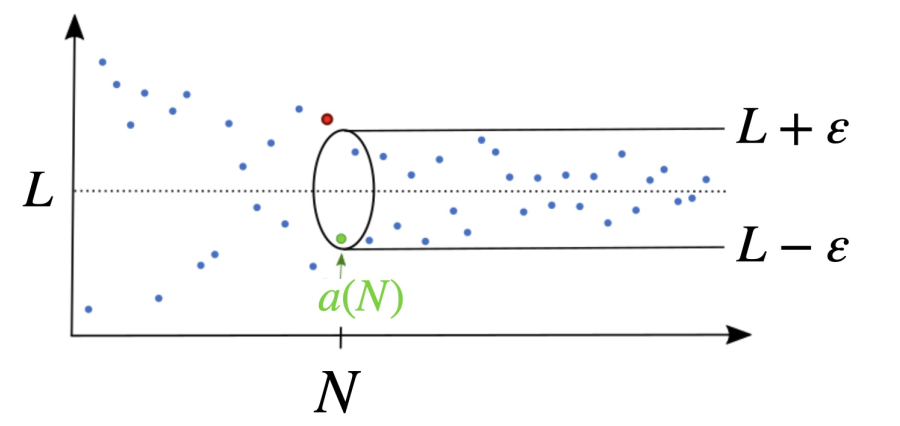
\includegraphics[width=0.5\linewidth]{fig/Convergencia.png}
\end{center}

Lo que hace que esta definición sea tan poderosa es su universalidad. El
Maquinista está esencialmente prometiendo: ``Dame cualquier requisito de
tolerancia, por estricto que sea, y puedo cumplirlo, aunque necesite más
recursos (un $N$ mayor) para especificaciones más ajustadas''.

Fíjate en algo más sobre la definición: no hace mención a que algo
suceda ``eventualmente'', o ``en el infinito'' ni ninguna otra palabra
ambigua y escurridiza. Hemos cambiado la ambigüedad de hablar del
infinito por la precisión de los cuantificadores existenciales y
universales. No más imprecisiones sobre lo que sucede ``cuando $n$ se
hace grande''; en su lugar, tenemos un desafío concreto: dada cualquier
tolerancia $\varepsilon$, ¿puedes encontrar un umbral específico $N$? Esa idea fue
el avance clave que permitió que el Cálculo entrara en el reino de las
matemáticas rigurosas.

En Lean, la definición se escribe así:

\begin{minted}{lean}
def LimSuc (a : ℕ → ℝ) (L : ℝ) : Prop :=
  ∀ ε > 0, ∃ N : ℕ, ∀ n ≥ N, |a n - L| < ε
\end{minted}

Esta sintaxis debería resultarte familiar por la táctica \texttt{have}
que ya conoces. El símbolo especial \texttt{def} (en lugar de
\texttt{have}) significa que estamos a punto de definir algo, y
\texttt{LimSuc} es su nombre (por \textit{Límite de Sucesión}, por
supuesto; pero podríamos haberlo llamado como quisiéramos). Luego
nuestras suposiciones son una sucesión \texttt{a : N -> R} y algún
número real \texttt{L : R}. Después de los dos puntos \texttt{:} va
nuestra salida, que en este caso es \texttt{Prop}, es decir, una
proposición (sentencia) que puede ser verdadera o falsa. Así que
\texttt{LimSuc} es en realidad una función que toma una sucesión y un
hipotético valor límite, y devuelve verdadero o falso dependiendo de si
se cumple la condición. Luego viene un signo de dos puntos e igual
\texttt{:=}, tras el cual se especifica la condición exacta que se va a
probar. Y la condición es lo que ya dijimos: para todo epsilon, .... La
gran diferencia es que puedes escribir \texttt{have} dentro de una
demostración, pero no puedes escribir \texttt{def} dentro de una;
\texttt{def} está reservado para crear definiciones globales a las que
se puede hacer referencia para siempre una vez introducidas.

Puede que te resulte útil una nueva táctica llamada \texttt{change}. Te
permite reemplazar un objetivo (o hipótesis) por algo que es
definicionalmente igual a él. En nuestro ejemplo, verás el objetivo como
\texttt{LimSuc a L}. ¿Qué se supone que debes hacer con eso? Bueno, si
recuerdas cómo se define \texttt{LimSuc}, entonces puedes reemplazar el
objetivo con la definición, escribiendo:

\begin{minted}{lean}
change ∀ ε > 0 , ∃ N : ℕ, ∀ n ≥ N , |a n - L| < ε
\end{minted}

Lean cambiará entonces el objetivo por su definición. Recuerda que
$\varepsilon, N$ y $n$ son todas variables mudas aquí, así que puedes divertirte
un poco:

\begin{minted}{lean}
change ∀ Alicia > 0 , ∃ Bob : ℕ, ∀ Blas ≥ Bob , |a Blas - L| < Alicia
\end{minted}

Y una última táctica que también podrías encontrar útil es
\texttt{norm\_num} (para normalizar valores numéricos); evalúa
expresiones numéricas y demuestra igualdades/desigualdades que
involucren números concretos. Por ejemplo, si te quedas atascado con un
$|0|$ en algún momento y quieres convertirlo en un simple $0$, intenta
llamar a \texttt{norm\_num}.

\begin{minted}{lean}
-- ---------------------------------------------------------------------
-- Demostrar que si a es una sucesión tal que para todo
-- n, a(n) = L, entonces a converge a L.
-- ----------------------------------------------------------------------

-- Demostración en lenguaje natural
-- ================================

-- Tenemos que demostrar que para cada ε ∈ ℝ tal que ε > 0, existe un
-- N ∈ ℕ, tal que (∀n ∈ ℕ)[n ≥ N → |a(n) - L| < ε]. Basta tomar N como
-- 0, ya que para todo n ≥ N se tiene
--    |a(n) - L| = |L - L|
--               = |0|
--               = 0
--               < ε

-- Demostraciones con Lean4
-- ========================

variable (a : ℕ → ℝ)
variable (L : ℝ)

-- 1ª demostración
-- ===============

example
  (h : ∀ n, a n = L)
  : LimSuc a L :=
by
  change ∀ ε > 0 , ∃ N : ℕ, ∀ n ≥ N , |a n - L| < ε
  -- ⊢ ∀ ε > 0, ∃ N, ∀ n ≥ N, |a n - L| < ε
  intro ε hε
  -- ε : ℝ
  -- hε : ε > 0
  -- ⊢ ∃ N, ∀ n ≥ N, |a n - L| < ε
  use 0
  -- ⊢ ∀ n ≥ 0, |a n - L| < ε
  intro n hn
  -- n : ℕ
  -- hn : n ≥ 0
  -- ⊢ |a n - L| < ε
  specialize h n
  -- h : a n = L
  rewrite [h]
  -- ⊢ |L - L| < ε
  ring_nf
  -- ⊢ |0| < ε
  norm_num
  -- ⊢ 0 < ε
  exact hε

-- 2ª demostración
-- ===============

example
  (h : ∀ n, a n = L)
  : LimSuc a L :=
by
  intros ε hε
  -- ε : ℝ
  -- hε : ε > 0
  -- ⊢ ∃ N, ∀ (n : ℕ), n ≥ N → |a n - L| < ε
  use 0
  -- ⊢ ∀ (n : ℕ), n ≥ 0 → |a n - L| < ε
  intros n hn
  -- n : ℕ
  -- hn : n ≥ 0
  -- ⊢ |a n - L| < ε
  show |a n - L| < ε
  calc |a n - L| = |L - L| := by rw [h n]
               _ = |0|     := by {congr ; exact sub_self L}
               _ = 0       := abs_zero
               _ < ε       := hε

-- 3ª demostración
-- ===============

example
  (h : ∀ n, a n = L)
  : LimSuc a L :=
by
  intros ε hε
  -- ε : ℝ
  -- hε : ε > 0
  -- ⊢ ∃ N, ∀ (n : ℕ), n ≥ N → |a n - L| < ε
  use 0
  -- ⊢ ∀ (n : ℕ), n ≥ 0 → |a n - L| < ε
  intros n hn
  -- n : ℕ
  -- hn : n ≥ 0
  -- ⊢ |a n - L| < ε
  show |a n - L| < ε
  calc |a n - L| = 0 := by simp [h n]
               _ < ε := hε

-- 4ª demostración
-- ===============

example
  (h : ∀ n, a n = L)
  : LimSuc a L :=
by
  intros ε hε
  -- ε : ℝ
  -- hε : ε > 0
  -- ⊢ ∃ N, ∀ (n : ℕ), n ≥ N → |a n - L| < ε
  aesop

-- 5ª demostración
-- ===============

example
  (h : ∀ n, a n = L)
  : LimSuc a L :=
by
  intros ε hε
  -- ε : ℝ
  -- hε : ε > 0
  -- ⊢ ∃ N, ∀ (n : ℕ), n ≥ N → |a n - L| < ε
  aesop

-- 6ª demostración
-- ===============

example
  (h : ∀ n, a n = L)
  : LimSuc a L :=
fun ε hε ↦ by aesop

-- Lemas usados
-- ============

#check (sub_self a : a - a = 0)
\end{minted}

¡Acabas de completar tu primera demostración rigurosa de un límite!
Reflexionemos sobre lo que has logrado y las ideas clave de este ejemplo
fundacional.

\textbf{Lo que acabas de demostrar:} Has demostrado que si una sucesión
siempre devuelve el mismo valor $L$, entonces converge a $L$. La
respuesta del Maquinista a cualquier demanda de tolerancia
$\varepsilon > 0$ es bellamente simple: ``¡Puedo cumplir esa especificación
inmediatamente con cualquier longitud de producción $N$, porque ya estoy
produciendo exactamente lo que quieres!''.

\textbf{Ideas clave de esta demostración:}
\begin{enumerate}
\item \textbf{La táctica \texttt{change}:} Aprendiste a desplegar una
  definición para ver qué es lo que realmente estás intentando
  demostrar. \texttt{LimSuc a L} se convirtió en la condición concreta
  epsilon-$N$.
\item \textbf{La estructura lógica:} La demostración siguió el flujo
  natural de la definición:
    \begin{itemize}
    \item \texttt{intro epsilon h\_epsilon} manejó el ``para todo
      $\varepsilon > 0$''.
    \item \texttt{use 1} proporcionó el testigo $N$ (¡cualquier número
      sirve!).
    \item \texttt{intro n hn} manejó el ``para todo $n \geq N$''.
    \item Luego la manipulación algebraica mostró que
      $|a(n) - L| = |L - L| = |0|$.
    \item Después, la normalización numérica dio que $|0| = 0$, y
      \texttt{h\_epsilon} finalmente demostró que $0 < \varepsilon$.
    \end{itemize}
\end{enumerate}

\textbf{La hermosa simplicidad:} Este es el escenario soñado por el
Maquinista: no importa cuán exigentes sean los requisitos de tolerancia
del ingeniero, la fábrica de constantes puede satisfacerlos
instantáneamente. ¡No hay compromiso entre precisión y esfuerzo porque
el resultado ya es perfecto!

Estás construyendo la base de todo el cálculo. Cada límite, derivada e
integral descansa en última instancia en argumentos como este.


Alejémonos un poco de la demostración formal de Lean y entendamos qué
acabamos de demostrar en lenguaje natural.

\begin{theorem}
  Si una sucesión tiene el mismo valor para cada término, entonces
  converge a ese valor constante.
\end{theorem}

\begin{proof}
  Supongamos que tenemos una sucesión $a(n)$ donde $a(n) = L$ para todo
  $n$, y queremos demostrar que esta sucesión converge a $L$.

  Por definición, necesitamos demostrar que para cualquier tolerancia
  $\varepsilon > 0$, podemos encontrar un punto $N$ tal que para todo
  $n \geq N$, tenemos $|a(n) - L| < \varepsilon$.

  Esto es casi trivialmente simple: como $a(n) = L$ para cada $n$,
  tenemos:
  \[ |a(n) - L| = |L - L| = |0| = 0 \]
  Como $0 < \varepsilon$ para cualquier $\varepsilon$ positivo, podemos elegir cualquier
  $N$ que queramos (elegimos $N = 1$ en la demostración, pero $N = 0$ o
  $N = 1000$ funcionarían igual de bien).

  Por lo tanto, para cualquier $n \geq N$, tenemos
  $|a(n) - L| = 0 < \varepsilon$, lo que demuestra la convergencia.
\end{proof}


%%% Local Variables:
%%% mode: LaTeX
%%% TeX-master: "Analisis_en_Lean"
%%% End:

\chapter{Convergencia de sucesiones}

\section{Más sobre sucesiones}

En el Tema 2, aprendimos la definición de una sucesión $a : \mathbb{N} \to \mathbb{R}$ que converge a un límite $L$: para cualquier tolerancia $\varepsilon > 0$, existe un momento $N$, de modo que, para cualquier punto posterior a ese momento, $n \ge N$, estamos dentro de la tolerancia, $|a_n - L| < \varepsilon$.

También aprendimos cómo hacer algo completamente trivial con ella, concretamente, demostrar que la sucesión constante converge, con esa constante como su límite. Vamos a subir un peldaño, ¿de acuerdo?


\section{Nivel 1: La propiedad arquimediana}

La llamada propiedad arquimediana (que creo que se debe originalmente a Eudoxo, y aparece ya en los \textit{Elementos} de Euclides, Libro V) es una propiedad fundamental de los números reales que captura la noción intuitiva de que no existen números reales positivos ``infinitamente grandes'' o ``infinitamente pequeños''.

Más precisamente, establece que no importa cuán pequeño sea $\varepsilon > 0$, siempre existe un número natural $N$ de modo que $1/N$ es aún más pequeño que $\varepsilon$ (y, por supuesto, positivo). Equivalentemente, podemos enunciarla como: para cualquier número real positivo $\varepsilon$, existe un número natural $N$ tal que $1/\varepsilon < N$.

\textit{¿Por qué importa esto?} La propiedad arquimediana es una de las propiedades más fundamentales que distinguen a los números reales de otros sistemas numéricos. Sin ella, podríamos tener números positivos ``infinitamente grandes'' o ``infinitamente pequeños'', lo que rompería la mayor parte del cálculo y el análisis.

Nuestro objetivo será demostrar lo siguiente:
\begin{theorem}[PropArq]
  Para cualquier $\varepsilon \in \mathbb{R}$ con $0 < \varepsilon$, existe $N \in \mathbb{N}$ tal que $1/\varepsilon < N$.
\end{theorem}

Esto es matemáticamente ``obvio'' para la mayoría de la gente: si tienes un número positivo $\varepsilon$, por muy pequeño que sea, siempre puedes encontrar un número natural lo suficientemente grande para que $1/\varepsilon$ sea menor que él. Pero, ¿cómo se formaliza esto realmente en Lean?

\subsection{La estrategia de demostración en lenguaje natural}

Primero, pensemos en esto en lenguaje natural. La clave es que necesitamos proporcionar un número natural $N$ específico que funcione.

Una opción natural sería utilizar algo relacionado con la función techo (\textit{ceiling}). La función techo $x \mapsto \lceil x \rceil$ redondea cualquier número real al entero más cercano por arriba. Sin embargo, hay un problema sutil aquí: la función techo estándar devuelve valores en los enteros $\mathbb{Z}$, pero necesitamos valores en $\mathbb{N}$ (los números naturales). ¡¡No son lo mismo!!

Afortunadamente, Lean proporciona la ``función techo de números naturales'', escrita como $x \mapsto \lceil x \rceil_+$, que toma cualquier número real y devuelve un número natural. (Puedes escribir estos símbolos usando \verb|\lceil|, \verb|\rceil| y \verb|\_+|). Para entradas negativas, esta función devuelve 0. Por ejemplo, $\lceil -3.14 \rceil_+ = 0$ y $\lceil 3.14 \rceil_+ = 4$.

Ahora nuestra estrategia queda clara:
\begin{itemize}
    \item \textbf{Elección de N:} Usar $N = \lceil 1 / \varepsilon \rceil_+ + 1$
    \item \textbf{Por qué funciona:} Tenemos la ``desigualdad clave'': $1 / \varepsilon \le \lceil 1 / \varepsilon \rceil_+$, que se cumple por la definición de la función techo.
    \item \textbf{Obtener la desigualdad estricta:} Sumar 1 nos da $1 / \varepsilon < \lceil 1 / \varepsilon \rceil_+ + 1$
\end{itemize}

\subsection{Los desafíos de la implementación en Lean}

En Lean, los dos primeros pasos de nuestra demostración en lenguaje natural funcionan bien, pero luego nos encontramos con el problema de la \textbf{coerción de tipos} (''casting'' entre diferentes tipos de números). Discutiremos esto con más detalle más adelante, pero de nuevo tiene que ver con el hecho de que $\mathbb{N}, \mathbb{Z}, \mathbb{Q}$ y $\mathbb{R}$ son todos tipos de cosas diferentes, y necesitamos poder mover los números hacia arriba en la jerarquía de ``sofisticación'', siendo los naturales los objetos más simples y los reales los más complicados.

Por ejemplo, fíjate en que cuando escribamos nuestra sentencia \texttt{have} para establecer la desigualdad clave:
\begin{minted}{lean}
have fact : 1 / ε ≤ ⌈1 / ε⌉₊ := by Demostracion
\end{minted}
Lean la registrará como:
\begin{minted}{lean}
fact : 1 / ε ≤ ↑ ⌈1 / ε⌉₊
\end{minted}
Observa la misteriosa flecha hacia arriba $\uparrow$. Esta representa una función de coerción de los números naturales a los reales:
\begin{center}
    $\uparrow : \mathbb{N} \to \mathbb{R}$
\end{center}
Esto se debe a que $\mathbb{N}, \mathbb{Z}, \mathbb{Q}$ y $\mathbb{R}$ son todos tipos \textbf{diferentes} en el sistema de tipos de Lean. Aunque pensemos que los naturales están ``contenidos'' en los reales, formalmente son tipos distintos, y Lean necesita funciones de coerción explícitas para convertir entre ellos.

Piénsalo de esta manera: el número natural $3 : \mathbb{N}$, la fracción $3/1 : \mathbb{Q}$ y el número real $3.000 : \mathbb{R}$ son objetos diferentes que simplemente representan el mismo valor matemático.

La táctica \texttt{push\_cast} ayuda a gestionar estas coerciones, de forma similar a \texttt{ring\_nf} pero para conversiones en lugar de operaciones de anillo.

\subsection{Nuevas herramientas que necesitarás}

\begin{itemize}
    \item $\lceil \cdot \rceil_+$: La función techo de números naturales.
    \item \texttt{push\_cast}: Táctica que maneja las coerciones entre tipos numéricos.
    \item \texttt{bound}: Resuelve muchas desigualdades rutinarias una vez que los tipos están correctamente alineados.
\end{itemize}

\subsection{Demostraciones en Lean}

\begin{minted}{lean}
import Mathlib.Data.Real.Basic
import Mathlib.Tactic

variable {ε : ℝ}
variable (h : 0 < ε)

-- Demostración en lenguaje natural
-- ================================

-- Sea N = ⌈1/ε⌉₊ + 1. Entonces,
--    1/ε ≤ ⌈1/ε⌉₊
--        < ⌈1/ε⌉₊ + 1
--        = N
-- Por lo tanto, 1/ε < N.

-- 1ª demostración
-- ===============

example : ∃ (N : ℕ), 1 / ε < N :=
by
  -- ⊢ ∃ N, 1 / ε < ↑N
  use ⌈1 / ε⌉₊ + 1
  -- ⊢ 1 / ε < ↑(⌈1 / ε⌉₊ + 1)
  have fact : 1 / ε ≤ ⌈1 / ε⌉₊ := by bound
  -- fact : 1 / ε ≤ ↑⌈1 / ε⌉₊
  push_cast
  -- ⊢ 1 / ε < ↑⌈1 / ε⌉₊ + 1
  bound

-- 2ª demostración
-- ===============

example : ∃ (N : ℕ), 1 / ε < N :=
by
  -- ⊢ ∃ N, 1 / ε < ↑N
  use ⌈1 / ε⌉₊ + 1
  -- ⊢ 1 / ε < ↑(⌈1 / ε⌉₊ + 1)
  have fact : 1 / ε ≤ ⌈1 / ε⌉₊ := Nat.le_ceil (1 / ε)
  -- fact : 1 / ε ≤ ↑⌈1 / ε⌉₊
  push_cast
  -- ⊢ 1 / ε < ↑⌈1 / ε⌉₊ + 1
  apply lt_of_le_of_lt fact
  -- ⊢ ↑⌈1 / ε⌉₊ < ↑⌈1 / ε⌉₊ + 1
  exact lt_add_one _

-- 3ª demostración
-- ===============

example : ∃ (N : ℕ), 1 / ε < N :=
by
  -- ⊢ ∃ N, 1 / ε < ↑N
  use ⌈1 / ε⌉₊ + 1
  -- ⊢ 1 / ε < ↑(⌈1 / ε⌉₊ + 1)
  push_cast
  -- ⊢ 1 / ε < ↑⌈1 / ε⌉₊ + 1
  calc
    1 / ε ≤ ↑⌈1 / ε⌉₊     := Nat.le_ceil (1 / ε)
    _     < ↑⌈1 / ε⌉₊ + 1 := lt_add_one _

-- 4ª demostración
-- ===============

example : ∃ (N : ℕ), 1 / ε < N :=
by
  -- ⊢ ∃ N, 1 / ε < ↑N
  use ⌈1 / ε⌉₊ + 1
  -- ⊢ 1 / ε < ↑(⌈1 / ε⌉₊ + 1)
  push_cast
  -- ⊢ 1 / ε < ↑⌈1 / ε⌉₊ + 1
  exact lt_of_le_of_lt (Nat.le_ceil (1 / ε)) (lt_add_one _)

-- 5ª demostración
-- ===============

example : ∃ (N : ℕ), 1 / ε < N :=
exists_nat_gt (1 / ε)

-- 6ª demostración
-- ===============

example : ∃ (N : ℕ), 1 / ε < N :=
by
  -- ⊢ ∃ N, 1 / ε < ↑N
  use ⌈1 / ε⌉₊ + 1
  -- ⊢ 1 / ε < ↑(⌈1 / ε⌉₊ + 1)
  calc
    1 / ε ≤ (⌈1 / ε⌉₊ : ℝ)     := Nat.le_ceil (1 / ε)
    _     < (⌈1 / ε⌉₊ : ℝ) + 1 := lt_add_one _
    _     = ↑(⌈1 / ε⌉₊ + 1)    := by norm_num

-- Lemas usados
-- ============

variable (a b c : ℝ)
#check (Nat.le_ceil a : a ≤ ↑⌈a⌉₊)
#check (exists_nat_gt (1 / ε) : ∃ n : ℕ, 1 / ε < ↑n)
#check (lt_add_one a : a < a + 1)
#check (lt_of_le_of_lt : a ≤ b → b < c → a < c)
\end{minted}

\subsection{Demostración en lenguaje natural de la propiedad arquimediana}

\begin{theorem}
  Para cualquier número real positivo $\varepsilon > 0$, existe un número natural $N$ tal que $1/\varepsilon < N$.
\end{theorem}

\begin{proof}
Sea $\varepsilon > 0$. Necesitamos encontrar un número natural $N$ tal que $1/\varepsilon <
N$.

Usamos el valor $N = \lceil 1/\varepsilon \rceil_+ + 1$, donde $\lceil \cdot \rceil_+$ denota la función
techo de números naturales.

Dado que $\varepsilon > 0$, tenemos $1/\varepsilon > 0$. Por la definición de la función techo de números naturales, sabemos que:
\[ 1/\varepsilon \le \lceil 1/\varepsilon \rceil_+ \]
Ahora, como $\lceil 1/\varepsilon \rceil_+$ es un número natural y $N = \lceil 1/\varepsilon \rceil_+ + 1$, tenemos:
\[ \lceil 1/\varepsilon \rceil_+ < \lceil 1/\varepsilon \rceil_+ + 1 = N \]
Combinando estas desigualdades, obtenemos:
\[ 1/\varepsilon \le \lceil 1/\varepsilon \rceil_+ < N \]
Por lo tanto, $1/\varepsilon < N$, lo que completa la demostración.
\end{proof}

\textbf{Significado:} La propiedad arquimediana es fundamental para el análisis porque asegura que los números reales no tienen elementos ``infinitos'' o ``infinitesimales''. Garantiza que siempre podemos encontrar números naturales lo suficientemente grandes como para dominar cualquier número real positivo dado cuando tomamos sus recíprocos. Esta propiedad es esencial para muchos procesos de límite y es equivalente a la completitud de los números reales en ciertas formulaciones.

\subsection{Revisión de errores comunes}
\begin{itemize}
    \item ¡No uses la función techo regular $\lceil \cdot \rceil$! ¡Devuelve enteros, no naturales!
    \item \textbf{Cuidado con los problemas de casting}: si \texttt{bound} no funciona, prueba \texttt{push\_cast} primero.
    \item La suma $\lceil 1/\varepsilon \rceil_+ + 1$ ocurre en $\mathbb{N}$, luego se convierte a $\mathbb{R}$; por eso necesitamos \texttt{push\_cast}.
\end{itemize}

\textbf{Nota histórica:} Aunque a menudo se atribuye a Arquímedes (c. 287-212 a.C.), esta propiedad probablemente era conocida por Eudoxo (c. 408-355 a.C.) y aparece en los \textit{Elementos} de Euclides. Arquímedes utilizó una versión de este principio en su método de exhaución para calcular áreas y volúmenes.

\section{Nivel 2: Nuestro primer límite real}

¡Enhorabuena! Acabas de demostrar la propiedad arquimediana. Ahora vamos a usarla para demostrar algo realmente interesante: nuestro primer límite no trivial.

\subsection{El objetivo: Demostrar que $1/n \to 0$}

Queremos demostrar que la sucesión $a(n) = 1/n$ converge a 0 cuando $n$ tiende a infinito. Esto es intuitivamente obvio: a medida que $n$ crece, $1/n$ se hace más pequeño y se acerca a 0. Pero, ¿cómo lo hacemos riguroso usando la definición $\varepsilon$-$N$?

\begin{theorem}
  La sucesión $a(n) = 1/n$ converge a 0.
\end{theorem}

\subsection{Recordatorio: La definición de convergencia de sucesiones}

Una sucesión $a : \mathbb{N} \to \mathbb{R}$ converge a un límite $L$ (escrito \texttt{LimSuc a L}) si:
\begin{itemize}
    \item Para cada $\varepsilon > 0$, existe $N : \mathbb{N}$ tal que para todo $n \ge N$, $|a(n) - L| < \varepsilon$
    \item En notación formal: $\forall \varepsilon > 0, \exists N, \forall n \ge N, |a(n) - L| < \varepsilon$
\end{itemize}
Para nuestro caso específico con $a(n) = 1/n$ y $L = 0$, esto se convierte en:
$\forall \varepsilon > 0, \exists N, \forall n \ge N, |1/n - 0| < \varepsilon$.

\subsection{Estrategia de demostración en lenguaje natural}

Así es como lo demostraremos paso a paso:
\begin{itemize}
    \item \textbf{Paso 1:} Sea $\varepsilon > 0$ dado. (Esto corresponderá a \texttt{intro $\varepsilon$ h$\varepsilon$}).
    \item \textbf{Paso 2:} Necesitamos encontrar un $N$ tal que para todo $n \ge N$, tengamos $1/n < \varepsilon$.
    \item \textbf{Idea clave:} Necesitamos $1/n < \varepsilon$, que es equivalente a $1/\varepsilon < n$ (ya que ambos lados son positivos). Así que necesitamos que $n$ sea mayor que $1/\varepsilon$.
    \item \textbf{Paso 3:} ¡Para eso desarrollamos la propiedad arquimediana! Nos dice que existe algún número natural $N$ tal que $1/\varepsilon < N$. En lugar de volver a demostrarlo desde cero, podemos simplemente citar este hecho; luego elegiremos tal $N$ y lo usaremos.
    \item \textbf{Paso 4:} Ahora sea $n \ge N$ dado. Tenemos:
    \begin{itemize}
        \item $1/\varepsilon < N$ (por nuestra elección de $N$)
        \item $N \le n$ (por hipótesis)
        \item Por lo tanto: $1/\varepsilon < N \le n$, así que $1/\varepsilon < n$
        \item Tomando recíprocos (y volteando la desigualdad): $1/n < \varepsilon$
    \end{itemize}
    \item \textbf{Paso 5:} Como $|1/n - 0| = |1/n| = 1/n < \varepsilon$, ¡hemos terminado!
\end{itemize}

\subsection{Los desafíos de la implementación en Lean}

\subsubsection{Desafío 1: Multiplicación cruzada de fracciones}
Nuestro paso clave es mostrar que $1/n < \varepsilon$. En matemáticas de papel, simplemente multiplicaríamos de forma cruzada para obtener $1 < n * \varepsilon$. Pero Lean es muy cuidadoso con la división por cero.
\textbf{Solución:} ¡La táctica \texttt{field\_simp} maneja esto automáticamente! Eliminará denominadores multiplicando de forma cruzada, pero solo después de verificar que todos los denominadores son positivos (o al menos no nulos).

\subsubsection{Desafío 2: Aritmética lineal}
Una vez eliminadas las fracciones, necesitamos combinar varias desigualdades. La táctica \texttt{bound} no siempre maneja bien estas combinaciones lineales con multiplicación por variables.
\textbf{Solución:} La táctica \texttt{linarith} está específicamente diseñada para la aritmética lineal. Puede tomar una lista de hipótesis y resolver metas que se sigan de combinaciones lineales de esas hipótesis.

\subsubsection{Desafío 3: Casting explícito de tipos}
¿Recuerdas las flechas hacia arriba $\uparrow$? ¡Han vuelto! Cuando escribimos $1/n$, Lean lo ve como $1/\uparrow n$ donde $n$ comienza como un número natural pero necesita ser convertido a real.
\textbf{Solución:} Podemos especificar el casting explícitamente con esta sintaxis: \texttt{(n : $\mathbb{R}$)}. Esto le dice a Lean exactamente a qué tipo queremos convertir $n$.

\subsubsection{Desafío 4: Casting en aplicaciones de tácticas}
A veces quieres aplicar una táctica pero los tipos no coinciden exactamente.
\textbf{Solución:} La táctica \texttt{exact\_mod\_cast} es como \texttt{apply}, pero maneja automáticamente las coerciones de tipo por ti.

\subsection{Nuevas herramientas que necesitarás}
\begin{itemize}
    \item \texttt{field\_simp}: Elimina denominadores.
    \item \texttt{linarith}: Potente táctica para desigualdades lineales.
    \item \texttt{exact\_mod\_cast}: Maneja coerciones automáticamente cuando la meta es exactamente la hipótesis tras el casting.
\end{itemize}

\subsection{Consejos profesionales para este nivel}
\begin{enumerate}
    \item Usa \texttt{change} para convertir \texttt{LimSuc a 0} a su definición.
    \item Aplica la propiedad arquimediana para obtener la existencia de $N$.
    \item Usa \texttt{choose} para extraer el $N$ de la sentencia existencial.
    \item Establece la positividad primero antes de usar \texttt{field\_simp}.
    \item Trabaja paso a paso.
\end{enumerate}

\subsection{Demostración en Lean}

\begin{minted}{lean}
Statement OneOverNLimZero ( a : $\mathbb{N}$ $\to$ $\mathbb{R}$) ( ha : $\forall$ n , a n = 1 / n ) :
  LimSuc a 0 := by
  change $\forall$ $\varepsilon$ > 0 , $\exists$ N , $\forall$ n $\ge$ N , | a n - 0| < $\varepsilon$
  intro $\varepsilon$ h$\varepsilon$
  have f1 : $\exists$ ( N : $\mathbb{N}$) , 1 / $\varepsilon$ < N := by apply PropArq h$\varepsilon$
  choose N eps_inv_lt_N using f1
  use N
  intro n n_ge_N
  ring_nf
  specialize ha n
  rewrite [ ha ]
  have f2 : |1 / ( n : $\mathbb{R}$) | = 1 / n := by bound
  rewrite [ f2 ]
  have f3 : 0 < 1 / $\varepsilon$ := by bound
  have Npos : (0 : $\mathbb{R}$) < N := by linarith [ f3 , eps_inv_lt_N ]
  have N_le_n : ( N : $\mathbb{R}$) $\le$ n := by exact_mod_cast n_ge_N
  have npos : (0 : $\mathbb{R}$) < n := by linarith [ Npos , N_le_n ]
  field_simp
  field_simp at eps_inv_lt_N
  have f4 : N * $\varepsilon$ $\le$ n * $\varepsilon$ := by bound
  linarith [ eps_inv_lt_N , f4 ]
\end{minted}

\subsection{Lo que acabamos de lograr}
Esta demostración demuestra varios conceptos clave:
\begin{enumerate}
    \item El poder de la propiedad arquimediana.
    \item La definición $\varepsilon$-$N$ en acción.
    \item Manipulación rigurosa de desigualdades.
    \item El puente entre la intuición y la formalidad.
\end{enumerate}

%%% Local Variables:
%%% mode: LaTeX
%%% TeX-master: "Analisis_en_Lean"
%%% End:


\end{document}

%%% Local Variables:
%%% mode: LaTeX
%%% TeX-master: t
%%% End:
